\chapter{\texorpdfstring{\lbz}{Lambdab} and \texorpdfstring{$\Lambda^0$}{Lambda} decay vertex reconstruction}
\label{cap:vertex_reconstruction}
This chapter details my work towards the improvement of the vertex reconstruction process for decays involving T tracks.
Section \ref{sec:reco_algorithms} delves into a deep study of the vertexing process at LHCb and the two algorithms employed in this thesis;
Section \ref{sec:reco_efficiency} introduces the problem of low vertexing efficiency for the decay of interest \demonstratorshort;
Section \ref{sec:characterization_non_converged} presents my efforts in the characterization of the non-converged events in search for the root cause of the vertexing falure;
Section \ref{sec:recovery_general} proposes my solution to improve the signal yield through partial recovery of non-reconstructed events;
finally, Section \ref{sec:lambda_endvertex_bias} features an analysis of \lambdadecay decay vertex resolution in the simulated signal dataset and a description of the main known sources of bias.
Section \ref{sec:3:cap3_conclusions} provides a short summary of the main results obtained in the chapter.

\section{Vertex reconstruction algorithms at LHCb}
\label{sec:reco_algorithms}

\subsection{Vertex Fitter algorithm}
The Vertex Fitter (VF) \cite{twiki_vf}, implemented as part of the LoKi analysis toolkit, is the main vertexing algorithm used for the reconstruction of the \lbz decay.

Under VF formalism, each daughter particle is represented by a 7-dimensional vector\footnote{This chapter assumes the standard right-handed LHCb coordinate system, see Section \ref{info:LHCb_system}.}
\begin{equation}
	\vec{p} = \begin{pmatrix}
		\vec{r} \\ \vec{q}
	\end{pmatrix}
	=
	\begin{pmatrix}
		r_x \\ r_y \\ r_z \\ p_x \\ p_y \\ p_z \\ E
	\end{pmatrix},
	\label{eq:particle_representation}
\end{equation}
containing its 4-momentum $\vec{q}$ computed at a certain reference point $\vec{r}$.
Parameter vector $\vec{p}$ has an associated covariance matrix $V$, which can be written in block structure as
\begin{equation}
	\begin{pmatrix}
		V_r      & V_{rq} \\
		V_{rq}^T & V_q
	\end{pmatrix}.
	\label{eq:par_covmatrix}
\end{equation}
It is also convenient to identify its formal inverse matrix $G := V^{-1}$, which has an analogous block form:
\begin{equation}
	\begin{pmatrix}
		G_r      & G_{rq} \\
		G_{rq}^T & G_q
	\end{pmatrix}
	=
	\begin{pmatrix}
		V_r      & V_{rq} \\
		V_{rq}^T & V_q
	\end{pmatrix}^{-1}
\end{equation}

Taking the daughter particles as inputs, the Vertex Fitter returns the best fit value $\vec{x}$ for the common origin vertex, along with its covariance matrix $C$ and the $\chi^2$ which can be used to evaluate the goodness of fit.

The algorithm builds the decay tree from the bottom up via a <<leaf-by-leaf>> approach, fitting one vertex at a time (e.g. $J/\psi \rightarrow \mu^+ \mu^-$, $\Lambda^0 \rightarrow p \pi^-$) and then moving upwards (e.g. $\Lambda_b^0 \rightarrow J/\psi\,\Lambda^0$).
The process is blind to the downstream leaves and only considers kinematic information of the immediate daughter particles, without accounting for momenta and mass constraints throughout the decay tree.

\subsubsection{Iterating paradigm}
The basic unit of recursion of the Vertex Fitter is the \textit{iteration}:
the algorithm is set to repeat the vertexing process until either a convergence condition is satisfied (see later) or the fit reaches the set number of allowed iterations, 10 by default.
In the latter case, a non-convergence error is thrown and the candidate event is discarded.

At the beginning of each iteration, the final vertex covariance matrix $C^{i-1}_n$ from the previous iteration\footnote{The subscript $n$ identifies the final step number, see later.} is scaled down by a factor $s^2 = {10}^{-4}$:
\begin{equation}
	C^{i}_0 = C^{i-1}_n \times s^2.
\end{equation}
The algorithm then performs a \textit{proper transportation}, a dedicated routine in which all daughter particles are extrapolated to the $z$ component of the current (tentative) position of the common production vertex $\vec{x}_n^{i-1}$.
%Such transportation is also performed at the end of the vertexing procedure to ensure an optimal computation of final particle momenta.

As mentioned in Section \ref{sec:2:tracking}, extrapolation using T tracks is a sensitive affair:
unlike the case for other track types, no constraints are available besides the downstream measurement performed by the T tracking stations, meaning the tracks have to be propagated through several meters while accounting for the intense and non-homogeneous LHCb magnetic field.
For this analysis, said extrapolation was performed via numerical solution of the track propagation equations using an approach based on the Runge-Kutta (RK) method \cite{Hairer1993}.
In the RK formalism, the track state at a given $z$ is parameterized with a five-dimensional representation
\begin{equation}
\vec{x} = \begin{pmatrix}
	x \\ y \\ t_x \\ t_y \\ \frac{Q}{P}
\end{pmatrix},
\end{equation}
with $t_{x} \coloneqq \frac{dx}{dz}$ (the same holds for $t_y$) and $\frac{Q}{P}$ is the charge-to-momentum ratio.
When extrapolating the track for a distance $\Delta z$, the new track state is computed with a fifth-order RK expansion
\begin{equation}
\vec{x}(\Delta z) = \vec{x}_0 + \sum_{m=1}^6 c_m \frac{d\vec{x}^m}{dz} \Delta z,
\end{equation}
with
\begin{equation}
\vec{x}^m = \sum_{n=1}^{m-1} b_{mn} \frac{d\vec{x}^n}{dz} \Delta z
\end{equation}
and Cash-Karp parameters $c_m$ and $b_{mn}$ chosen to obtain a precision of $(\Delta z)^6$ \cite{Bos:1070314}.



% @todo: explain Runge-Kutta, a che ordine?

%---
%
%When all particles have been added, i.e. all steps have been performed, the algorithm concludes an \textit{iteration}.
%The process is then repeated 
%
%Within an individual iteration, the vertex position is updated at each step following \eqref{eq:VF_new_vertex_final}.
%Consequently, the individual momenta of the particles must also be updated to reflect the change in reference point;
%this is performed with a degree of approximation in equation \eqref{eq:VF_new_momentum_final}.
%To supplement this, every iteration begins with a \textit{proper transportation}

%\subsubsection{Old}
%
%combining the position $\vec{x}$ of the estimated origin vertex of the track (known as \textit{reference point}) with the  of the track constrained to originate in $\vec{x}$.
%At the end of the fitting process,  will coincide with the common vertex chosen for all daughter particles.
%
%In the VF framework it's sometimes useful to write vector particle vector $\vec{p}_k$ in terms of $\vec{x}_k$ and $\vec{q}_k$ via a projection matrix formalism:
%\begin{equation}
%	\vec{p}_k = c^0_k + A_k \vec{x}_k + B_k \vec{q}_k,
%\end{equation}
%with $A_k$ and $B_k$ defined as
%\begin{equation}
%A_k = \left[
%	\frac{\partial \vec{p}_k}{\partial \vec{x}_k}
%\right],
%\quad\quad 
%B_k = \left[
%	\frac{\partial \vec{p}_k}{\partial \vec{q}_k}
%\right].
%\end{equation}
%Of course, the simple representation described in \eqref{eq:particle_representation} allows for likewise simple projection matrices:
%\begin{equation}
%A_k = A = \begin{pmatrix}
%1 \\
%0
%\end{pmatrix},
%\quad\quad 
%B_k = B = \begin{pmatrix}
%0 \\
%1
%\end{pmatrix}.
%\end{equation}
%
%--

\subsubsection{Step}
Within an individual iteration $i$, denoted by a superscript, the Vertex Fitter algorithm proceeds by \textit{steps} denoted by subscripts, with each step $k$ coinciding with the addition of the $k$-th daughter particle.

Given information on the vertex position $\vec{x}_{k-1}$ obtained using the first $k-1$ particles, track $k$ is added through the following recursive procedure.
First the inverse vertex covariance matrix is updated:
\begin{equation}
{(C^i_k)}^{-1} = {(C^i_{k-1})}^{-1}
+
%{(V_k^i)}_r^{-1},
{(G_k^i)}_r
\label{eq:3:VF_new_inv_covmatrix}
\end{equation}
where the reference point inverse covariance matrix ${(G_k^i)}_r = {(V_k^i)}_r^{-1}$ has been updated at the beginning of the iteration as part of the the proper transportation.

%\begin{equation}
%G_k^B = G_k - G_k B_k W_k B_k^T G_k.
%\end{equation}
%The above auxiliary matrix depends from the particle parameter inverse covariance matrix $G_k$, extrapolated at the current vertex position (see the next paragraph), as well as from the matrix
%and
%\begin{equation}
%W_k = {\left(B_k^T G_k B_k\right)}^{-1}.
%\end{equation}

%After this, $C_k^{-1}$ is inverted and the algorithm updates the correlation matrix $E_k \coloneqq \text{corr}(\vec{x}_{k},\vec{q}_k)$ between vertex position and $k$-th particle momentum
%\begin{equation}
%E_k = -F_k C_k
%\end{equation}
%and the momentum covariance matrix
%\begin{equation}
%D_k = W_k - E_k F_k^T,
%\end{equation}
%with
%\begin{equation}
%F_k = W_k B_k^T G_k A_k.
%\end{equation}

If ${(C^i_k)}^{-1}$ can successfully be inverted, the algorithm updates the current best estimate of the common origin vertex by combining information from the previous step ($\vec{x}_{k-1}^i$) with information from the properly transported current particle (reference point $\vec{r}_k^i$ from representation \eqref{eq:particle_representation}) through the associate inverse covariance matrices:
\begin{equation}
\vec{x}_k^i = C_k^i \left[
	{(C^i_{k-1})}^{-1} \vec{x}_{k-1}^i
	+ {(G_k^i)}_r \vec{r}_k^i
\right].
\label{eq:VF_new_vertex_final}
\end{equation}
%with $\vec{r}_k^i$ being the reference point from representation \eqref{eq:particle_representation}.
New vertex $\vec{x}_k^i$ doubles as reference point for the $k$-th particle until the next transportation, ergo track momentum is also updated to match it\footnote{In this equation, $\coloneqq$ stands for the assignment operator.}
\begin{equation}
	\vec{q}_k^i \coloneqq
	\vec{q}_k^i
	-
	{(V_k^i)}_{rq}
	{(G_k^i)}_r
	\left(
		\vec{r}_k^i - \vec{x}_k^i
	\right).
	\label{eq:VF_momentum_final}
\end{equation}

To conclude the step, the vertex $\chi^2$ is updated to the account for the new position:
\begin{equation}
\begin{aligned}
	{(\chi^2)}_k^i &= {(\chi^2)}_{k-1}^i \\
	&+
	{\left(\vec{r}_{k}^i - \vec{x}_k^i\right)}^T  {(G_k^i)}_r \left(\vec{r}_{k}^i - \vec{x}_k^i \right) \\
	&+
	{\left(\vec{x}_k^i - \vec{x}_{k-1}^i\right)}^T  {(C_{k-1}^i)}^{-1} \left(\vec{x}_k^i - \vec{x}_{k-1}^i\right) \\
\end{aligned}.
\label{eq:VF_vertex_chi2_final}
\end{equation}

%Finally the step concludes with the computation of a new estimated vertex position
%\begin{equation}
%\vec{x}_k = C_k \left[
%	C_{k-1}^{-1} \vec{x}_{k-1}
%	+
%	A_k^T G_k^B \left(
%		\vec{p_k} - c_k^0	
%	\right)
%\right],
%\end{equation}
%a new 4-momentum for the $k$-th track
%\begin{equation}
%\vec{q}_k = W_k B_k^T G_k \left[
%	\vec{p_k} - c_k^0 - A_k \vec{x}_k
%\right],
%\end{equation}
%and an updated $\chi^2$ to evaluate the goodness of the best fit value for the decay vertex
%\begin{equation}
%\begin{aligned}
%\chi^2_k &= \chi^2_{k-1} \\
%&+
%\left[
%	\vec{p} - c_k^0 - A_k \vec{x}_k - B_k\vec{q}_k
%\right]^T G_k \left[
%	\vec{p} - c_k^0 - A_k \vec{x}_k - B_k\vec{q}_k
%\right] \\
%&+
%\left[
%	\vec{x}_k - \vec{x}_{k-1}
%\right] C_{k-1}^{-1} \left[
%	\vec{x}_k - \vec{x}_{k-1}
%\right]
%\end{aligned}.
%\end{equation}

%So far...
%
%\begin{equation}
%G_k = \begin{pmatrix}
%G_x 		&& G_{xp} \\
%G^T_{xp} 	&& G_p
%\end{pmatrix}
%\end{equation}
%
%\begin{equation}
%W_k = G_p^{-1}
%\end{equation}
%
%\begin{equation}
%G_k^B = \begin{pmatrix}
%G_x - G_{xp}G_p^{-1}G_{xp}^T 	&& 0 \\
%0								&& 0
%\end{pmatrix}
%\end{equation}
%
%\begin{equation}
%F_k = G_p^{-1} G_{xp}^T
%\end{equation}
%
%\begin{equation}
%C_k^{-1} = C_{k-1}^{-1} + \left[
%	G_x - G_{xp}G_p^{-1}G_{xp}^T
%\right]
%\end{equation}
%
%\begin{equation}
%E_k = -G_p^{-1} G_{xp}^T C_k
%\end{equation}
%
%\begin{equation}
%D_k = G_p^{-1} + G_p^{-1} G_{xp}^T C_k G_{xp} G_p^{-1}
%\end{equation}
%
%
%
%\begin{equation}
%\vec{q}_k = \begin{pmatrix}
%	G_p^{-1} G_{xp}^T && 0
%\end{pmatrix}
%\left[
%	\vec{p_k} - c_k^0 - A\vec{x}_k
%\right]
%\label{eq:VF_new_momentum_final}
%\end{equation}
%
%\begin{equation}
%\begin{pmatrix}
%	G_x && G_{xp} \\
%	G_{xp}^T && G_p
%\end{pmatrix}
%=
%\begin{pmatrix}
%	V_x && V_{xp} \\
%	V_{xp}^T && V_p
%\end{pmatrix}^{-1}
%\end{equation}
%
%\begin{subequations}
%\begin{align}
%&G_x - G_{xp} G_p^{-1} G_{xp} 	= V_x^{-1} \\
%&G_p^{-1} 						= V_p - V_{xp}^T V_x^{-1} V_{xp} \\
%&G_p^{-1} G_{xp}^T 				= -V_{xp}^T V_x^{-1}
%\end{align}
%\end{subequations}

\subsubsection{Seeding}
\label{sec:3:seeding}

The recursive procedure requires, at each step, a previous estimated vertex position $\vec{x}_{k-1}^i$, an associated inverse covariance matrix ${(C_{k-1}^i)}^{-1}$ and a ${(\chi^2)}_{k-1}^i$. In particular, step $k=1$ demands the existence of $\vec{x}_0^i$, ${(C_{0}^i)}^{-1}$ and ${(\chi^2)}_{0}^i$.

For iterations $i>1$, such roles are filled by the final vertex computed during the previous iteration.
This leaves out the crucial $i=1,k=1$ step;
to make up for it, at the beginning the algorithm extracts a \textit{vertex seed}, a first estimate of the decay vertex position, through a dedicated procedure depending on decay topology and properties of particles involved.

In the case of interest of the \lambdadecay two-body decay, said procedure is a single simplified iteration that uses the initial $\vec{p}$ track measurement performed by the T stations:
\begin{subequations}
\begin{align}
	&{(C_{0}^{1})}^{-1} = \sum_{j=p,\pi} {G_r}_j, \\
	&\vec{x}_0^1 = C_0^1 \sum_{j=p,\pi} {G_r}_j \vec{r}_j.
\end{align}
\end{subequations}
%with subscripts $1$ and $2$ referring to the two daughter particles in the decay (i.e. proton and pion).
Update of momenta is handled in the same way as equation \eqref{eq:VF_momentum_final}.
A new $\chi^2_0$ is computed for each particle:
\begin{subequations}
\begin{align}
	{{(\chi^2)}_0^1}_{(p)} &= 
	{\left(\vec{r}_{p} - \vec{x}_0^1\right)}^T  {G_r}_p \left(\vec{r}_{p} - \vec{x}_0^1 \right), \\
	{{(\chi^2)}_0^1}_{(\pi)} &= 
	{\left(\vec{r}_{\pi} - \vec{x}_0^1\right)}^T  {G_r}_\pi \left(\vec{r}_{\pi} - \vec{x}_0^1 \right),
\end{align}
\end{subequations}
conventionally choosing ${(\chi^2)}_0^1 \coloneqq {{(\chi^2)}_0^1}_{(p)}$.

\subsubsection{Termination and smoothing}
The two VF convergence conditions are both based on comparisons between the vertex position computed at the end of the current iteration with the one from the previous iteration, with convergence being called if either one of them is satisfied.

The first condition is placed on the absolute distance between the vertices:
\begin{equation}
	\left\|
	\vec{x}_n^{i} - \vec{x}_n^{i-1}
	\right\| \leq d_1
	\label{eq:cond_conv_1}
\end{equation}
where $d_1 = \SI{1}{\micro\meter}$ by default.
The second condition, by far the one more commonly satisfied when reaching convergence using T tracks\footnote{This doesn't happen using Long tracks, suggesting that the $d_1 = \SI{1}{\micro\meter}$ threshold is too strict given the scale of uncertainties in T station measurements. Nevertheless, increasing $d_1$ does not improve the vertex reconstruction efficiency discussed in Section \ref{sec:reco_efficiency}.}, concerns vertex distance <<in $\chi^2$ units>>:
\begin{equation}
	{\left(
	\vec{x}_n^{i} - \vec{x}_n^{i-1}
	\right)}^T
	{(C_n^i)}^{-1}
	\left(
	\vec{x}_n^{i} - \vec{x}_n^{i-1}
	\right)
	\leq d_2
	\label{eq:cond_conv_2}
\end{equation}
with $d_2 = 0.01$.
While condition \eqref{eq:cond_conv_1} can be satisfied at any point in the vertexing process, \eqref{eq:cond_conv_2} additionally requires $i>1$, excluding the very first iteration.

When convergence is reached at iteration $N$, the algorithm applies a smoothing process: for each daughter particle $k$, the reference point $\vec{r}_k$ is fixed to the final vertex position $\vec{x}_n^{N}$ and momentum $\vec{q}_k$ is updated accordingly as
\begin{equation}
	\vec{q}_k =
	\vec{q}_k^N
	-
	{(V_k^N)}_{rq}
	{(G_k^N)}_{r}
	\left(
		\vec{r}_k^N - \vec{x}_n^N
	\right),
\end{equation}
with $\vec{r}_k^N$ being the last computed reference point with related $\vec{q}_k^N$.

Last comes the evaluation of the relevant covariance matrices. The vertex covariance matrix $C$ is obviously fixed at $C_n^N$;
the algorithm also computes for each entry the correlation matrix $E_k \coloneqq \text{corr}\left(\vec{x_n^N},\vec{q}_k\right)$ between the vertex position and the particle momentum
\begin{equation}
	E_k = - F_k C,
	\label{eq:Ek}
\end{equation}
and the particle $\vec{q}_k$ covariance matrix
\begin{equation}
	D_k =
	{(V_k^N)}_q
	-
	{(V_k^N)}_{rq}
	{(G_k^N)}_r
	{(V_k^N)}_{rq}^T
	+
	F_k C F_k^{-1},
	\label{eq:Dk}
\end{equation}
with
\begin{equation}
	F_k =
	- {V_{rq}}_k {V_r}_k^{-1}
	\label{eq:Fk}
\end{equation}
being an auxiliary matrix.

\subsubsection{Mother particle creation}
Assuming the found vertex is inside the LHCb fiducial volume, the fit is validated and a $\chi^2$ is determined by taking the last step value from \eqref{eq:VF_vertex_chi2_final} and adding the $\chi^2$ from any short-lived daughter particle.
Degrees of freedom (DOFs) for $\chi^2$ reduction are computed as follows:
\begin{itemize}
	\item each track contributes 2 DOFs;
	\item each $\rho^+$-like particle\footnote{A $\rho^+$-like particle is a particle resulting from the combination of 1 long-lived particle and $\geq 2$ photons. The category identifier is owed to the topology of the $\rho^+ \rightarrow \pi^+\pi^0$ decay with $\pi^0 \rightarrow \gamma \gamma$.} contributes 2 DOFs;
	\item each sub-vertex contributes 3 DOFs plus further DOFs from the downstream decay tree;
	\item the sum total is reduced by 3. %% Perché?
\end{itemize}

A mother particle is subsequently created using the \eqref{eq:particle_representation} representation with reference point $\vec{x}_\text{mother}$ fixed to the new-found vertex coordinates.
Its 4-momentum is computed as a simple sum of the 4-momenta of its daughters extrapolated at the vertex:
\begin{equation}
	\vec{q}_\text{mother} = \sum_{k \in \text{daughters}} \vec{q}_k.
\end{equation}

The parameter vector covariance matrix \eqref{eq:par_covmatrix} is determined as follows:
\begin{equation}
	V_{r}^\text{mother} = C,
\end{equation}
\begin{equation}
	V_{q}^\text{mother} = \sum_{k \in \text{daughters}} \left[
		D_k
		+
		\sum_{\substack{j\in\text{daughters} \\ j \neq k}}
		\left(
			F_k C F_j^T + F_j C F_k^T
		\right)
	\right],
\end{equation}
\begin{equation}
	V_{rq}^\text{mother} = \sum_{k \in \text{daughters}} E_k,
\end{equation}
with $D_k$, $E_k$ and $F_k$ for each daughter resulting from \eqref{eq:Dk}, \eqref{eq:Ek} and \eqref{eq:Fk} respectively.

Finally, the mother particle measured mass $M_\text{mother}$ is computed as magnitude of 4-vector $\vec{q}_\text{mother}$ in the $(-,-,-,+)$ metric
\begin{equation}
	M_\text{mother} = \sqrt{E_\text{mother}^2
	- {p_x}_\text{mother}^2
	- {p_y}_\text{mother}^2
	- {p_z}_\text{mother}^2
	},
\end{equation}
Its associated uncertainty is defined as
\begin{equation}
	\sigma_M^\text{mother} = \sqrt{
		\frac{1}{4 M_\text{mother}^2}
		v^T
		H
		v
	},
\end{equation}
with
\begin{equation}
	v \coloneqq \frac{dM_\text{mother}^2}{d\vec{q}}
	= \begin{pmatrix}
		-2 {p_x}_\text{mother} \\
		-2 {p_y}_\text{mother} \\
		-2 {p_z}_\text{mother} \\
		2 E_\text{mother}
	\end{pmatrix}
\end{equation}
and
\begin{equation}
	H \coloneqq \sum_{k \in \text{daughters}} {V_q}_k.
\end{equation}

\subsection{Decay Tree Fitter algorithm}
\label{sec:3:dtf}
While the leaf-by-leaf approach adopted by the Vertex Fitter is fast, it brings alongside it the significant drawback of forgoing upstream information when fitting the downstream branches of a decay.
This is especially notable for decays like $K_S^0 \rightarrow \pi^0\pi^0 \rightarrow \gamma\gamma\gamma\gamma$, where the final state has no tracks to form a vertex with.
Even in the relatively more traditional case of the $\Lambda_b^0 \rightarrow J/\psi\,\Lambda^0$ decay, however, the VF algorithm still limits our options.
In particular, it prevents the placing of \textit{mass constraints} on mother particles, where the fit fixes the invariant mass of daughter pair to the PDG value for mother particle mass.

To compensate for this, all reconstructed events in this analysis undergo a refit process based on the Decay Tree Fitter (DTF) algorithm \cite{Hulsbergen:2005pu} first developed in BaBar.
This algorithm fits the entire decay chain simultaneously, fixing the decay vertices to the values found by the Vertex Fitter, and allows to place mass constraints on $p\pi^-$ and $\mu^+\mu^-$ invariant masses to match $m(\Lambda^0)$ and $m(J/\psi)$ respectively.

%% @todo: Ci starebbe un bel test in cui confronti la distribuzione dei vertici VF e DTF per mostrare che sono uguali (lo sono, vero??). Devi estrarli via Kinematic, immagino, perché nel rootfile non ci sono.

%\begin{figure}[t]
%	\centering
%	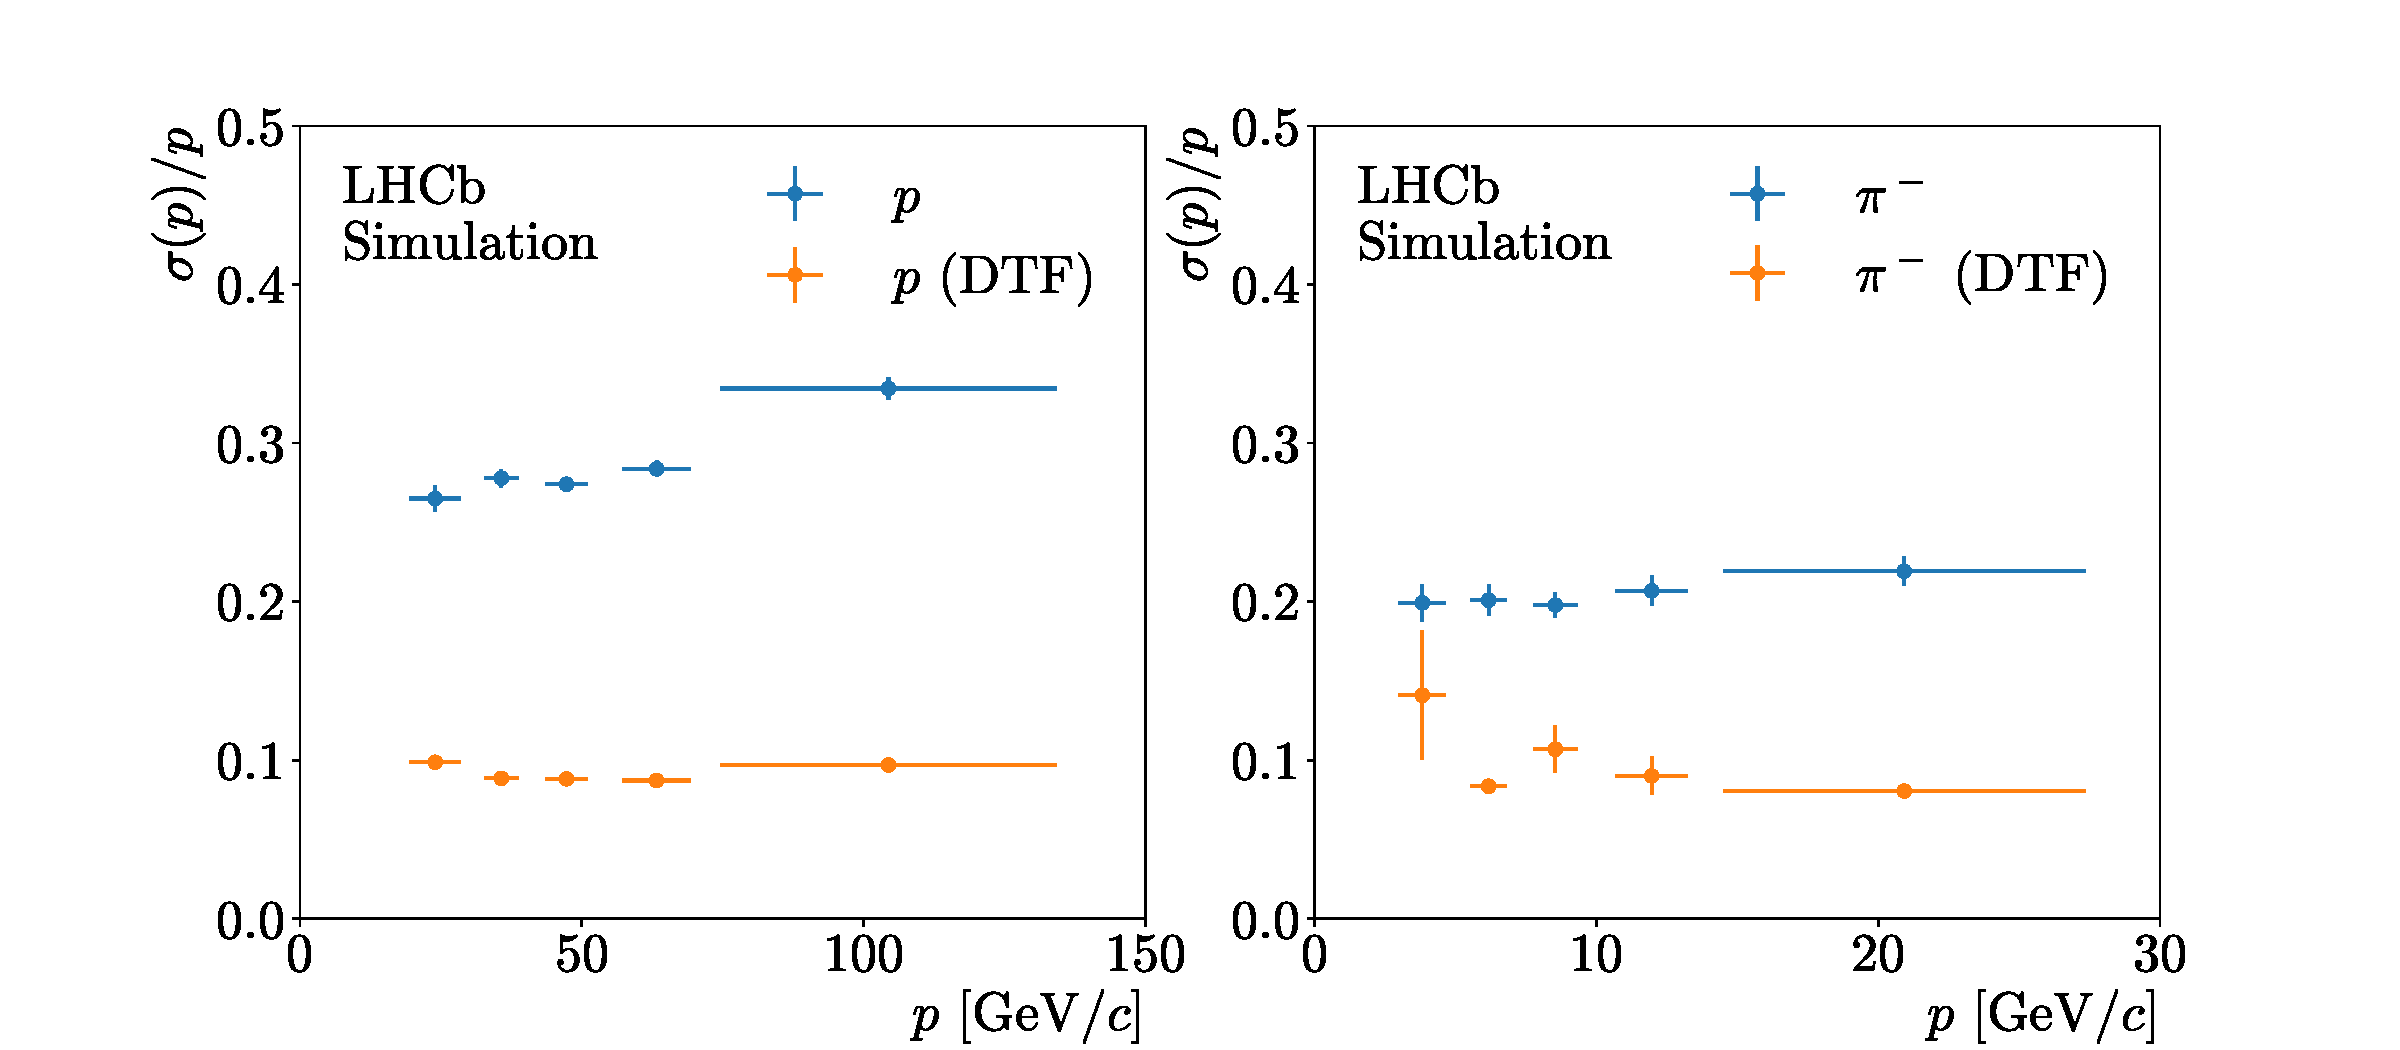
\includegraphics[width=\textwidth]{graphics/04-event_selection/paper_momentum_resolutions.pdf}
%	\caption[Momentum resolution.]{Momentum resolution.}
%	\label{fig:paper_momentum_resolutions}
%\end{figure}

While this step introduces another filtering process and related efficiency to account for\footnote{DTF convergence efficiency with the double mass constraint is relatively uneven across the $z_\Lambda^\textbf{vtx}$ spectrum, starting at $\approx 50\%$ for $z_\Lambda^\textbf{vtx} \approx \SI{6}{\meter}$ and growing up to $\approx 85\%$ for $z_\Lambda^\textbf{vtx} \approx \SI{7.5}{\meter}$.
Comparatively, vertex reconstruction is still the primary cause of event loss in this analysis.}, it proves invaluable for our physics motivations as it mitigates the most problematic drawback of T track usage, momentum resolution:
using both \jpsi and \lz mass constraints improves $\vec{p}$ resolution from $20$--$30\%$ to $\approx 10\%$ for protons and pions alike.
%As shown in Figure \ref{fig:paper_momentum_resolutions},
%Using both \jpsi and \lz mass constraints improves $\vec{p}$ resolution from $20$--$30\%$\footnote{Pion momentum resolution is higher because the pion receives a smaller fraction of the \lz momentum, thereby having a larger bending curve than the proton and allowing for better momentum measurement at the T stations.} to $\approx 10\%$.

%% Con KineAtVtx non è più vero.
%For the purposes of the helicity angle analysis outlined in Section \ref{sec:lambda}, particle momenta computed with the DTF algorithm are particularly valuable because, in addition to their greater accuracy, they are provided directly at the production vertex;
%by contrast, VF momenta are provided either at the decay vertex (short-lived particles) or at the position of first measurement (long-lived or stable particles).

\section{Reconstruction efficiency of the \texorpdfstring{$\Lambda^0_b$}{Lambdab} and \texorpdfstring{\lz}{Lambda} decays}
\label{sec:reco_efficiency}

To compute the vertex reconstruction efficiency for the \lbz decay chain, it is useful to conceptualize our event selection as a five step process:
\begin{enumerate}
	\item reconstruction of associated tracks for all charged daughter particles;
	\item reconstruction of \lz and \lbz decay vertices\footnote{\jpsi vertex reconstruction is is a prerequisite for event selection in the detached $J/\psi\rightarrow \mu^+ \mu^-$ trigger line (see Section \ref{sec:2:used_data}) and does not factor in the vertexing efficiency.};
	\item preliminary selections based on kinematic variables to filter out most background (see Section \ref{sec:prefilter});
	\item Decay Tree Fitter refit with appropriate mass constraints for the analysis at hand (usually \jpsi and \lz);
	\item further selections applied to events passing all previous steps. Detailed in Chapter \ref{cap:event_selection}, these include physical background vetoes and signal selection via a trained multivariate classifier.
\end{enumerate}

For the purposes of this section, we are interested in the first two steps (track and vertex reconstruction).

Efficiencies are computed with respect to \textit{reconstructible} particles, a flag attributed during the simulation process based on the number of hits (charged clusters with defined positions) in specific modules of the LHCb detector.
A track is said to be reconstructible as VELO track with hits in $\geq 3$ VELO modules, while it's reconstructible as T track with $\geq 1$ hits in both the $x$ and stereo layers of each T station.
If these conditions are satisfied simultaneously, the track qualifies for reconstructibility as Long track \cite{Li:2752971}.

At Monte Carlo level, a track is deemed to be \textit{reconstructed} if it can be successfully matched to at least one MC particle;
for T and Long tracks, this is true if at least $70\%$ of the hits from the respective relevant detectors for reconstructibility are shared between reconstructed and true track. For \demonstratorshort events with a true $z_\text{vtx}^\Lambda \in [\SI{6.0}{\meter}, \SI{7.6}{\meter}]$, this results in a track reconstruction efficiency
\begin{equation}
	\varepsilon_\text{reconstruction} \coloneqq \frac{n_\text{reconstructed}}{n_\text{reconstructible}}
\end{equation}
in the 60\% to 80\% range.

\begin{figure}[t!]
	\centering
	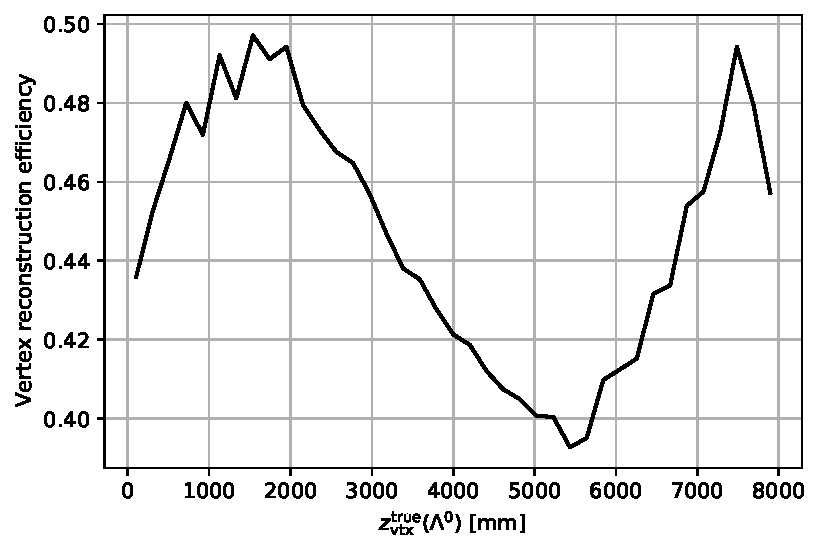
\includegraphics[width=.6\textwidth]{graphics/03-vertex_reconstruction/lambda_lambdab_reco_efficiency.pdf}
	\caption[A]{Reconstruction efficiency of simulated $\Lambda^0_b \rightarrow J/\psi~(\rightarrow \mu^+\mu^-)~\Lambda^0~(\rightarrow p\pi^-)$ events as function of the $z$ component of the true \lz decay vertex. Given that $J/\psi \rightarrow \mu^+ \mu^-$ events are reconstructed as part of the trigger step, the low efficiency is attributed to failure in reconstructing \lz and \lbz decay vertices.}
	\label{fig:lambda_lambdab_reco_efficiency}
\end{figure}

When considering how many of these reconstructed charged particles pass the vertex reconstruction (\textit{vertexing}) process, efficiency
\begin{equation}
	\varepsilon_\text{vertexing} \coloneqq \frac{n_\text{vertexed}}{n_\text{reconstructed}}
\end{equation}
is much lower.
Figure \ref{fig:lambda_lambdab_reco_efficiency} plots \lbz and \lz vertexing efficiency through the whole true $z_\text{vtx}^\Lambda$ spectrum, showing it never manages to get past the 50\% threshold.
This means that over half of candidate signal events are lost during the second step of the five-step selection process.

Available information does not distinguish between \demonstratorshort and \lambdadecay vertexing efficiencies.
Nevertheless, the rare usage of T tracks for physics analysis in LHCb suggests that problems are likelier to arise in the \lambdadecay vertexing and then cascade into \demonstratorshort reconstruction.
In the following sections I'll thus focus on the \lambdadecay decay with the goal of understanding the problem and improving signal yield.


\section{Characterization of non-converged events}
\label{sec:characterization_non_converged}
In order to narrow down the possible origin of the vertexing deficiency in \lambdadecay events, I conducted a series of comparative studies to characterize non-converged events and their differences to reconstructed ones.
The full simulated \demonstratorshort dataset constructed for the measurement of the \lz electromagnetic dipole moments omits a lot of technical information on the decays, the retention of which would make storage and quick access impractical.
Furthermore, a lot of the work in this and the next sections required direct changes to the vertexing algorithm for debugging and event recovery, which in turn required data to be reprocessed.
For these reasons, the studies in the following sections were conducted on a smaller sample of $\approx 110\,000$ \lbz decays (about 4600 of which are reconstructed) in $\sign{B_y} = +1$ configuration, where $\vec{B}$ is the LHCb magnetic field.

\subsection{Decay kinematics before and after interaction with the detector}
\label{sec:3:kinematics_at_first_meas}
%To gather information on the possible sources of the oscillating behaviour outlined in Section \ref{sec:oscillation}, I investigated the collective properties of a sample of \demonstratorshort decays in search of significant discrepancies between converged and failed events.
No difference between converged and failed \demonstratorshort events emerges at Monte Carlo level when considering the true values of basic kinematic variables such as daughter particle momenta and decay vertices locations of the three unstable particles \lbz, \lz and \jpsi.
Moreover, there doesn't seem to be a critical decay geometry associated to the drop in vertexing efficiency;
for instance, there is no evidence that \lambdadecay decays lying largely in the $xz$ plane, a setup quite unfriendly to the VF algorithm (see Section \ref{sec:lambda_endvertex_bias}), have any disproportionate representation amongst non-converged events.
This rules out the hypothesis that the failure of vertex fit convergence be caused by particle characteristics at production, such as protons and pions with unusually low transverse momentum \pt.

I also considered the possibility that kinematic asymmetries between converged and failed events may arise after interaction with the LHCb detector;
one example of this would be the case where failed events correlate with hits in a specific sections of the IT or OT trackers.
To this end I studied the event \textit{protoparticles}, data structures created during the LHCb event reconstruction process to encapsulate relevant information for the associated particle:
particle identification from the RICH and muon detectors, results from calorimeter hits and track information.

\begin{figure}[t]
	\centering
	\begin{subfigure}{.45\textwidth}
		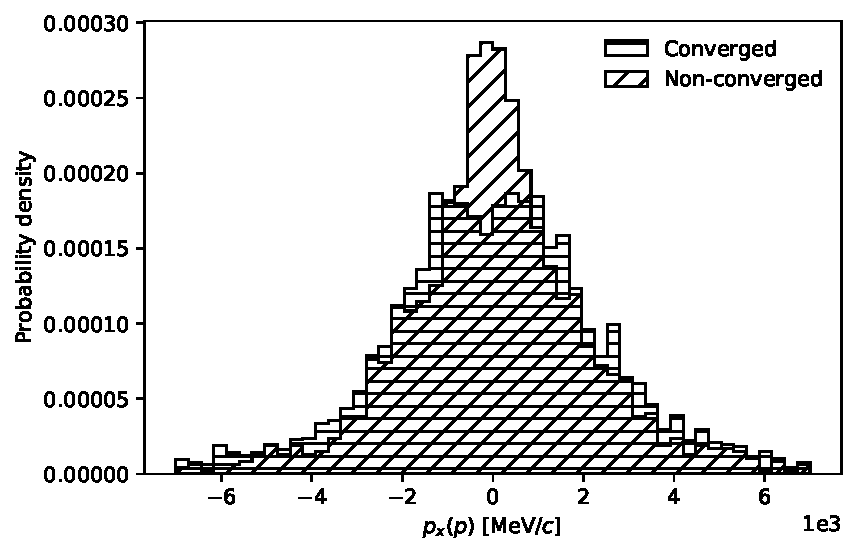
\includegraphics[width=\textwidth]{graphics/03-vertex_reconstruction/p_momentum_x.pdf}
		\caption{}
		\label{fig:3:p_momentum_x}
	\end{subfigure}
	\begin{subfigure}{.45\textwidth}
		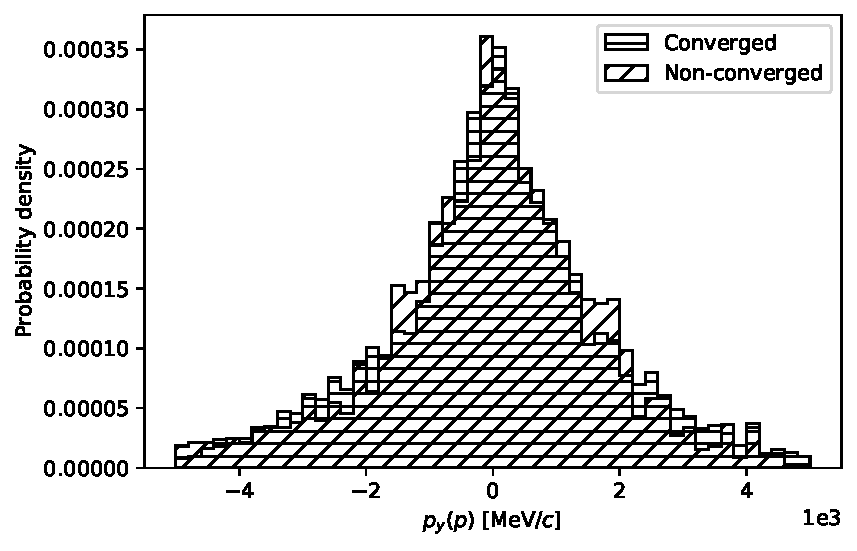
\includegraphics[width=\textwidth]{graphics/03-vertex_reconstruction/p_momentum_y.pdf}
		\caption{}
		\label{fig:3:p_momentum_y}
	\end{subfigure}
	\caption{Normalized distributions of proton protoparticles $p_x$ \textit{(a)} and $p_y$ \textit{(b)} components in simulated \lambdadecay events. Distributions of events with converging vertex fit are depicted with \textit{horizontal hatching}, non-converging fit with \textit{diagonal hatching}.}
	\label{fig:3:p_protoparticle_momenta}
\end{figure}

Charged protoparticles in particular store momentum and energy evaluated in a certain reference point which, for stable particles, corresponds to the position of first measurement of the track.
Figure \ref{fig:3:p_momentum_x} depicts the only major discrepancy between converged and failed events I found in the protoparticle analysis:
non-converged \lbz decays have a proton protoparticle $p_x$ distribution concentrated in $p_x \approx 0$, while converged decays show even dispersion of the central peak in the $[-\SI{1}{\gev},\SI{1}{\gev}]$ region.
This contrasts with $p_y$, the other component of the protoparticle transverse momentum, whose two distributions are almost overlapping (Figure \ref{fig:3:p_momentum_y}).
%While statistics in the reduced samples are too low to say for sure,
Pions do not appear to show similar discrepancies in their protoparticles.
Given the significant overlap between the distributions in Figure \ref{fig:3:p_momentum_x}, however, the overabundance of low $p_x$ of proton protoparticles in non-converged events does not appear to be a deciding factor for the Vertex Fitter failure.

%Assuming $p_x$ measurement at detector level is not biased, this result suggests that protons from failed events have generally lower $p_x$ when they reach the T stations;
%this would not be apparent from \pt distributions at the point of production, since the final $p_x$ value depends on the bending radius imprinted by the magnet (which in turn depends on momentum and distance traveled).
%Such low values of $p_x$ are potentially more susceptible to poor measurement by the T stations, which in turn affects the overall momentum resolution based on the particle bending radius in the $xz$ plane.

%Low values of $p_x$ imply roughly perpendicular incidence in the $xz$ bending plane used for momentum measurement by the T stations, which would affect the already poor momentum resolution 
%
%The correlation between low proton protoparticle $p_x$ and vertexing failure contains a valuable hint:
%converged and failed events may not differ in \pt of protons and pions at the point of productions, but it's possible that they do at the point of first measurement, after the particles are bent by the magnet.
%
%Poor measurement of $p_x$
%
%A precise estimate of $p_x$ is of paramount importance for correct track measurement and extrapolation:
%even slight mistakes in angle assessment are magnified during particle transportation through long distances, especially since the T track requirement leaves no upstream constraints.
%Moreover, momentum itself is computed through evaluation of the particle bending curve in the $xz$ plane induced by the magnet.
%As such, \lambdadecay events with low $p_x (p)$ when the proton reaches the T stations would be more suscetible to poor momentum measurement and 
%
%The link between 
%
%
%As such, one possible interpretation of the correlation between proton protoparticle $p_x$ and failure in vertexing is that 
%One possible interpretation is thus that
%
%As such, it stands to reason that poor measurement of the low proton $p_x$ can have enough of an effect to throw off the vertexing algorithm.

\subsection{Behaviour through VF iterations}
\label{sec:oscillation}
The VF process reaches convergence if either condition \eqref{eq:cond_conv_1} or \eqref{eq:cond_conv_2} is satisfied, i.e. if the vertex position estimated at iteration $i$ and the one from iteration $i-1$ are <<close enough>> either in absolute distance or $\chi^2$ distance, up until $i_\text{max} = 10$.
This is predicated on the principle that the algorithm refines its vertex estimate after each iteration, homing in on the candidate vertex with the lowest $\tilde{\chi}^2_\text{vtx}$.

Such a behaviour is not found in non-converging (henceforth also known as \textit{failed}) events.
This can be seen by increasing $i_\text{max}=100$, which causes a negligible $\approx 2\%$ increase in converged events.
It follows that, for the vast majority of missing events, failure of convergence is not a product of low computation time and must instead result from some internal malfunction of the vertexing process.

\begin{figure}[t]
	\centering
	\begin{subfigure}{.45\textwidth}
		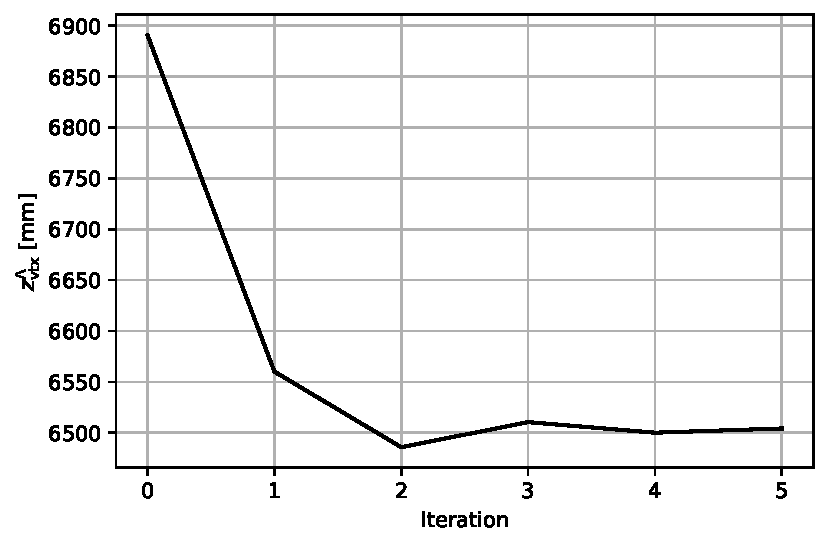
\includegraphics[width=\textwidth]{graphics/03-vertex_reconstruction/evt0_vertex_z.pdf}
		\caption{}
		\label{fig:z_iter_conv}
	\end{subfigure}
	\begin{subfigure}{.45\textwidth}
		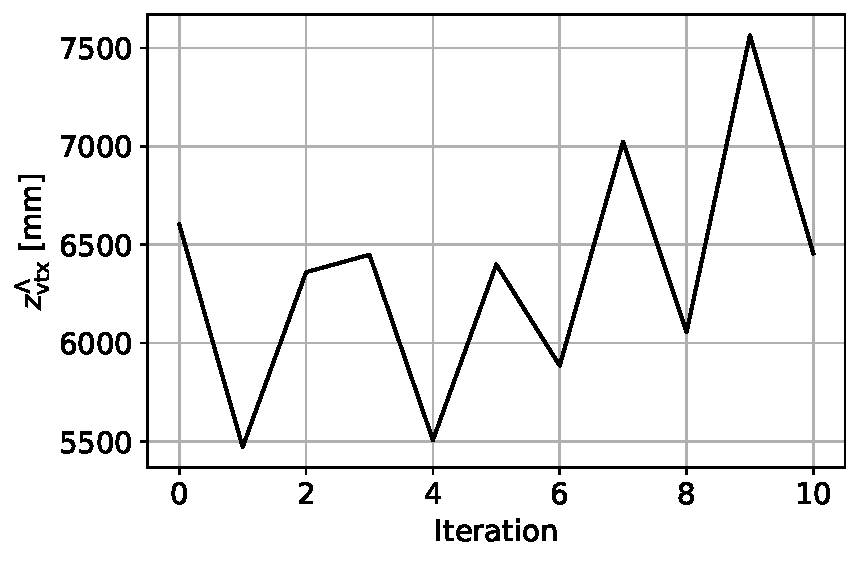
\includegraphics[width=\textwidth]{graphics/03-vertex_reconstruction/evt83_vertex_z.pdf}
		\caption{}
		\label{fig:z_iter_failed}
	\end{subfigure}
	\caption{Best values of tentative \lambdadecay vertex $z$ component at the end of each Vertex Fitter iteration for examples of converged \textit{(a)} and failed \textit{(b)} events.}
	\label{fig:z_iter_conv_vs_failed}
\end{figure}

This becomes apparent when studying the vertex positions throughout the iterating process for instances of converged and failed events of simulated signal.
Figure \ref{fig:z_iter_conv_vs_failed} compares the values of $z_\text{vtx}^\Lambda$, the $z$ component of the \lambdadecay decay vertex, as reconstructed by the VF in iterations $i=0$ to $10$ ($i=0$ being the starting seed).
Figure \ref{fig:z_iter_conv} (converged) exhibits the expected behaviour, with the algorithm refining its vertex estimate after every iteration and finally converging as early as $i=5$.
By contrast, Figure \ref{fig:z_iter_failed} (failed) presents an oscillating behaviour of $z_\text{vtx}^\Lambda$, swinging by as much as \SI{1}{\meter} in the opposite direction after an iteration completes.
While a particularly tricky instance of the first type of event may potentially benefit by an increased $i_\text{max}$, no amount of allotted computations can lead the second type to convergence.

\begin{figure}[t]
	\centering
	\begin{subfigure}{.45\textwidth}
		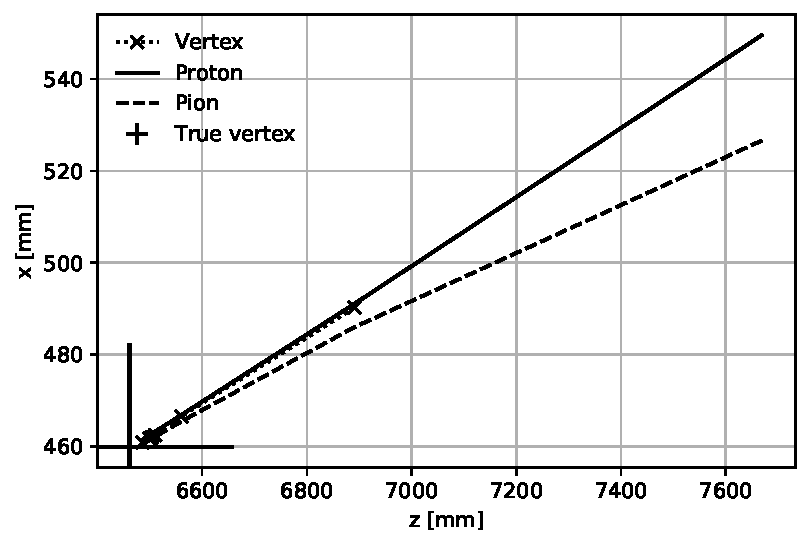
\includegraphics[width=\textwidth]{graphics/03-vertex_reconstruction/evt_0_zx.pdf}
		\caption{}
		\label{fig:3:converged_zx}
	\end{subfigure}
	\begin{subfigure}{.45\textwidth}
		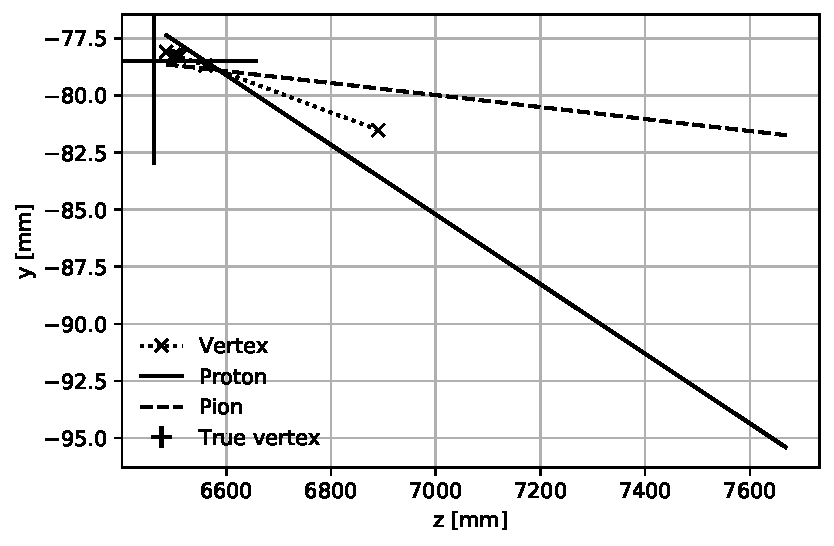
\includegraphics[width=\textwidth]{graphics/03-vertex_reconstruction/evt_0_zy.pdf}
		\caption{}
		\label{fig:3:converged_zy}
	\end{subfigure}
	\caption{\lambdadecay decay topology for an instance of converged event, projected in the $xz$ \textit{(a)} and $yz$ \textit{(b)} planes.
	The temporary best vertex locations chosen by the Vertex Fitter at the end of each iterations are marked with \textit{diagonal crosses} and linked by the \textit{dotted line} in iteration order (the second iteration best vertex is connected to the first, the third to the second and so on).
	The reconstructed vertex, while not explicitly represented, can be identified by the cluster of vertex point markers.
	At the beginning of each iteration, daughter particles are extrapolated at the $z$ of the best vertex of the previous iteration: proton (\textit{solid line}) and pion (\textit{dashed line}) tracks are drawn joining the respective reference points after transportation in order of decreasing $z$ (i.e. not in iteration order).
	The true vertex is marked by the \textit{large Greek cross}.}
	\label{fig:3:converged_event_topology}
\end{figure}

We can gain more insight into the nature of this oscillation by approaching the problem from a more topological point of view.
Figure \ref{fig:3:converged_event_topology} shows the topology of the converged event from Figure \ref{fig:z_iter_conv} in the bending $xz$ and non-bending $yz$ planes.
While the points of closest distance between the tracks in the two planes are not exactly matched, the algorithm manages to converge on a vertex position that is reasonably close to the true generated decay vertex.

\begin{figure}[t]
	\centering
	\begin{subfigure}{.45\textwidth}
		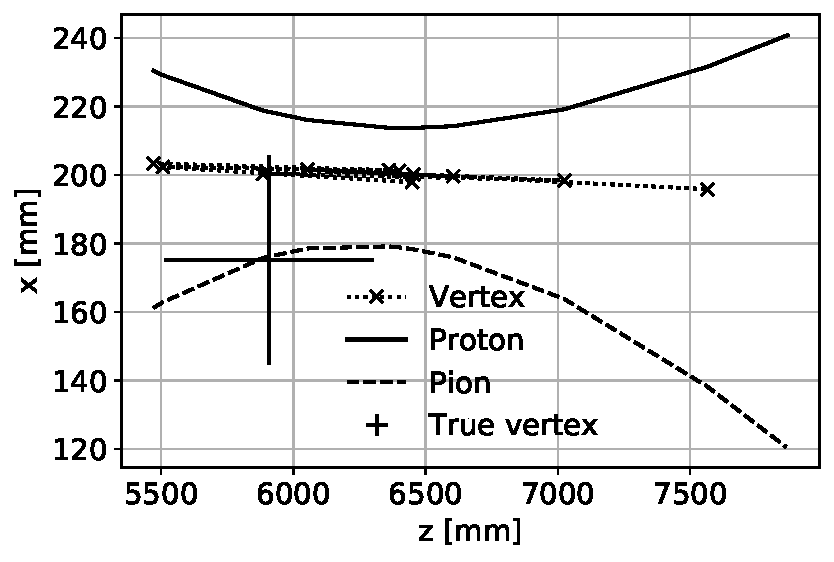
\includegraphics[width=\textwidth]{graphics/03-vertex_reconstruction/evt_83_zx.pdf}
		\caption{}
		\label{fig:3:failed_zx}
	\end{subfigure}
	\begin{subfigure}{.45\textwidth}
		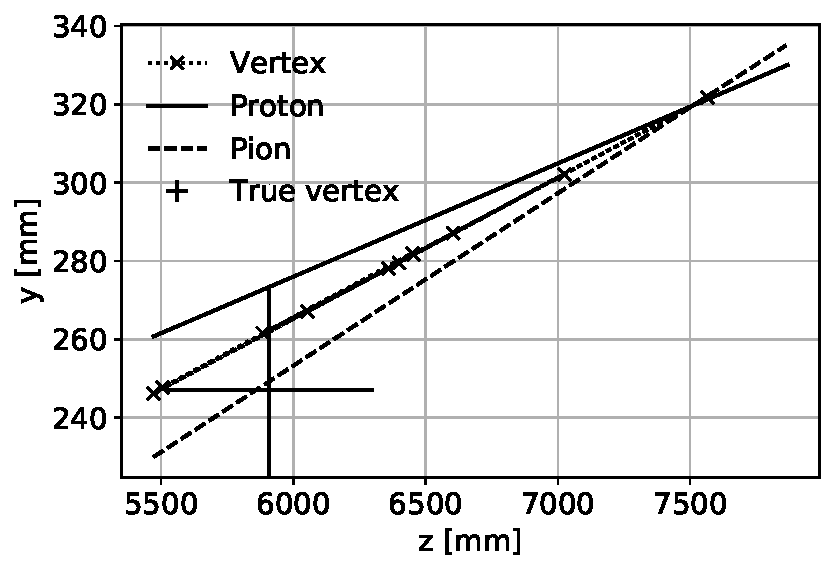
\includegraphics[width=\textwidth]{graphics/03-vertex_reconstruction/evt_83_zy.pdf}
		\caption{}
		\label{fig:3:failed_zy}
	\end{subfigure}
	\caption{\lambdadecay decay topology for an instance of non-converged event, projected in the $xz$ \textit{(a)} and $yz$ \textit{(b)} planes.
	Notation follows the one in Figure \ref{fig:3:converged_event_topology}.}
	\label{fig:3:failed_event_topology}
\end{figure}

The behaviour for the non-converged event from Figure \ref{fig:z_iter_failed}, shown in Figure \ref{fig:3:failed_event_topology}, is drastically different.
The dotted line following the best vertex estimate through iterations in the bending plane (Figure \ref{fig:3:failed_zx}) shows that the algorithm gravitates \textit{around} the point of closest distance between proton and pion tracks ($z \approx \SI{6.25}{\meter}$), never outright choosing it as candidate.
On the other hand, in the $yz$ plane (Figure \ref{fig:3:failed_zy}) the two tracks cross at a much more downstream point ($z \approx \SI{7.5}{\meter}$), which the Vertex Fitter also largely ignores during the iteration process.

%Some more insight into the nature of this oscillation can be achieved by taking a more <<geometrical>> look, plotting inter-iteration vertex coordinates in the $zx$ plane where the LHCb magnet bends tracks according to their charge.
%Figure \ref{fig:zx_iter_conv_vs_failed} compares the same events from Figure \ref{fig:z_iter_conv_vs_failed}.
%Again, the converged event in Figure \ref{fig:zx_iter_conv} behaves as intended, selecting as vertex roughly the point of closest distance between the tracks (some leeway is accorded since the fit also incorporates information from $xy$ and $yz$ planes).
%The progress in Figure \ref{fig:zx_iter_failed} is more interesting: in the failed case the estimated vertex, identified at each iteration by <<x>> markers along the dashed line, appears to gravitate \textit{around} the point of closest distance, never outright choosing it as candidate.
%Significantly, the \textit{true} $\Lambda^0$ vertex (marked by the green cross) lags some \SI{50}{\centi\meter} behind it.


\begin{figure}[t]
	\centering
	\begin{subfigure}{.45\textwidth}
		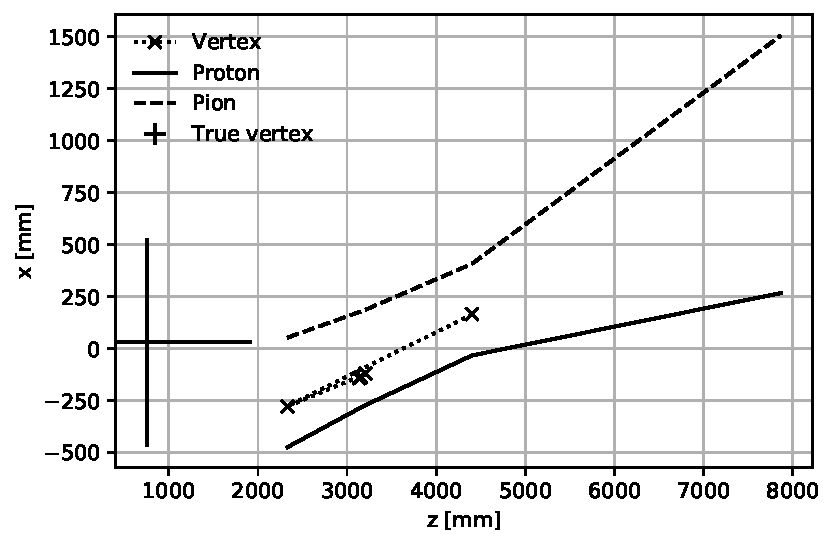
\includegraphics[width=\textwidth]{graphics/03-vertex_reconstruction/evt_6_zx.pdf}
		\caption{}
		\label{fig:3:converged_detached_zx}
	\end{subfigure}
	\begin{subfigure}{.45\textwidth}
		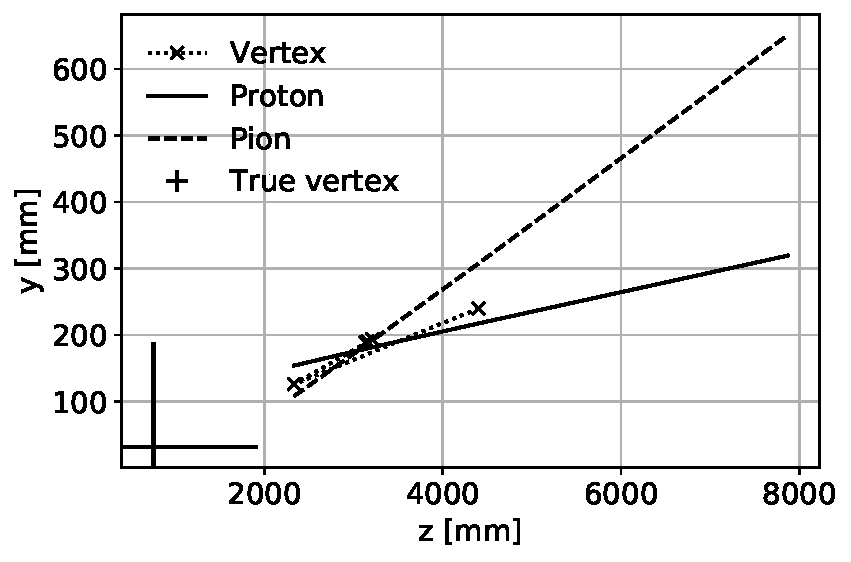
\includegraphics[width=\textwidth]{graphics/03-vertex_reconstruction/evt_6_zy.pdf}
		\caption{}
		\label{fig:3:converged_detached_zy}
	\end{subfigure}
	\caption{\lambdadecay decay topology for an instance of converged event with large track gap in the $xz$ plane, projected in the $xz$ \textit{(a)} and $yz$ \textit{(b)} planes.
	Notation follows the one in Figure \ref{fig:3:converged_event_topology}.}
	\label{fig:3:converged_detached_event_topology}
\end{figure}

Failed convergence in this event cannot be attributed to the comparatively larger gap between proton and pion tracks at their point of closest distance in the bending plane.
The VF algorithm has shown to be capable of bridging an imperfect track extrapolation: the converged event shown in Figure \ref{fig:3:converged_detached_event_topology} has a closest track distance of some \SI{40}{\centi\meter}, an order of magnitude greater than the track distance seen in Figure \ref{fig:3:failed_event_topology}.
Despite the large gap, the VF is able to recognize $z \approx \SI{3}{\meter}$ as the best candidate for the vertex.
This happens despite the large distance between this point and the true \lambdadecay vertex:
the discrepancy is due to poor initial momentum measurement for the tracks and demonstrates the flexibility of the VF algorithm, converging even in circumstances that are far from ideal.

%While it may be tempting to attribute the failed convergence to the comparatively larger gap between proton and pion tracks at their point of closest distance, some observations are in order:
%first, the deceivingly different $x$ scales in Figures \ref{fig:zx_iter_conv} and \ref{fig:zx_iter_failed} mean that in the latter tracks are closer than they may seem;
%more to the point, the VF algorithm has shown to be capable of bridging an imperfect track extrapolation in converged events, as demonstrated in Figure \ref{fig:zx_iter_conv_backstep}.

The more convincing explanation for the vertex oscillation is therefore that the candidate vertices in the $xz$ and $yz$ planes are too far apart for the VF to reconcile the two; the algorithm is not equipped to favour one over the other, leading to meter-wide swings when it strays too far off from either of them.
Convergence failure in Figure \ref{fig:3:failed_event_topology} can thus be interpreted through the lens of \textit{conflicting information}.

In this section I have focused the analysis on one particular event for didactic purposes.
%For didactic purposes, the analysis in this section has focused on just one event.
All the outlined patterns are nonetheless commonplace throughout failed events I have examined, with the oscillating vertex behaviour in particular being a constant in all of them.
While it would be reckless to conclude that every \lambdadecay vertexing failure must be the fault of $xz$ and $yz$ track mismatch, I have been able to use these findings, along with other from the following paragraphs, to devise a partial solution in Section \ref{sec:blowup_matrix}.

%\subsection{True kinematics}
%To further investigate the possible source of the oscillating behaviour outlined in Section \ref{sec:oscillation}, I have conducted a systematic comparison of kinematic features at Monte Carlo level between converged and failed events.
%
%No difference among the two categories emerge when considering basic decay descriptors such as the momenta of all particles involved and the decay vertices of unstable particles.
%Moreover, there doesn't seem to be a critical decay geometry that triggers the vertexing;
%for instance, there is no evidence that $\Lambda^0 \rightarrow p\pi^-$ decays lying largely in the $xz$ plane, a setup quite unfriendly to the VF algorithm (see Section \ref{sec:lambda_endvertex_bias}), has any disproportionate representation amongst non-converged events.
%
%\subsection{Kinematics at first measurement position}
%\label{sec:3:kinematics_at_first_meas}
%A major discrepancy emerges when looking at particle interaction with the detector via \textit{protoparticles}.
%A protoparticle is a data structure created during the LHCb event reconstruction process with the intent of encapsulating all relevant information available for the associated particle:
%particle identification (PID) from the RICH and muon detectors, results from calorimeter hits and track information.
%The latter contains details on momentum in relation to a certain reference point which, for stable charged particles, corresponds to the position of first measurement.
%
%\begin{figure}[t]
%	\centering
%	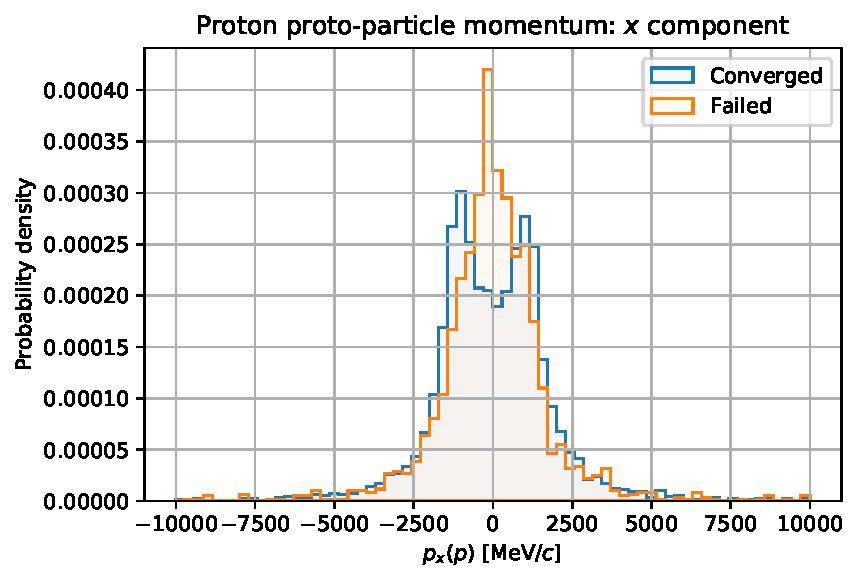
\includegraphics[width=.6\textwidth]{graphics/03-vertex_reconstruction/pp_p_momentum_x.pdf}
%	\caption{A.}
%	\label{fig:pp_p_px_conv_vs_failed}
%\end{figure}
%
%In the case of simulated protons from $\Lambda_b^0 \rightarrow J/\psi\,\Lambda^0$ decays, the distribution of the
%%true\footnote{While protoparticles result from interaction of the particle with the material, at this point I'm specifically considering the true value of the first measurement position and related momentum. Later on we'll instead delve into the \textit{reconstructed} counterparts of these quantities, which can be different as a result of poor T station measurements.}
%protoparticle $p_x$ for converged and failed events shows a marked difference outlined in Figure \ref{fig:pp_p_px_conv_vs_failed}:
%correctly reconstructed events tend to have a double peak roughly centered in $\approx \pm \SI{1}{\gev}$, while missing events have a more traditional single peak centered in $0$.
%
%%% todo: spezza in due? Fixa anche il testo poco dopo.
%\begin{figure}[t]
%	\centering
%	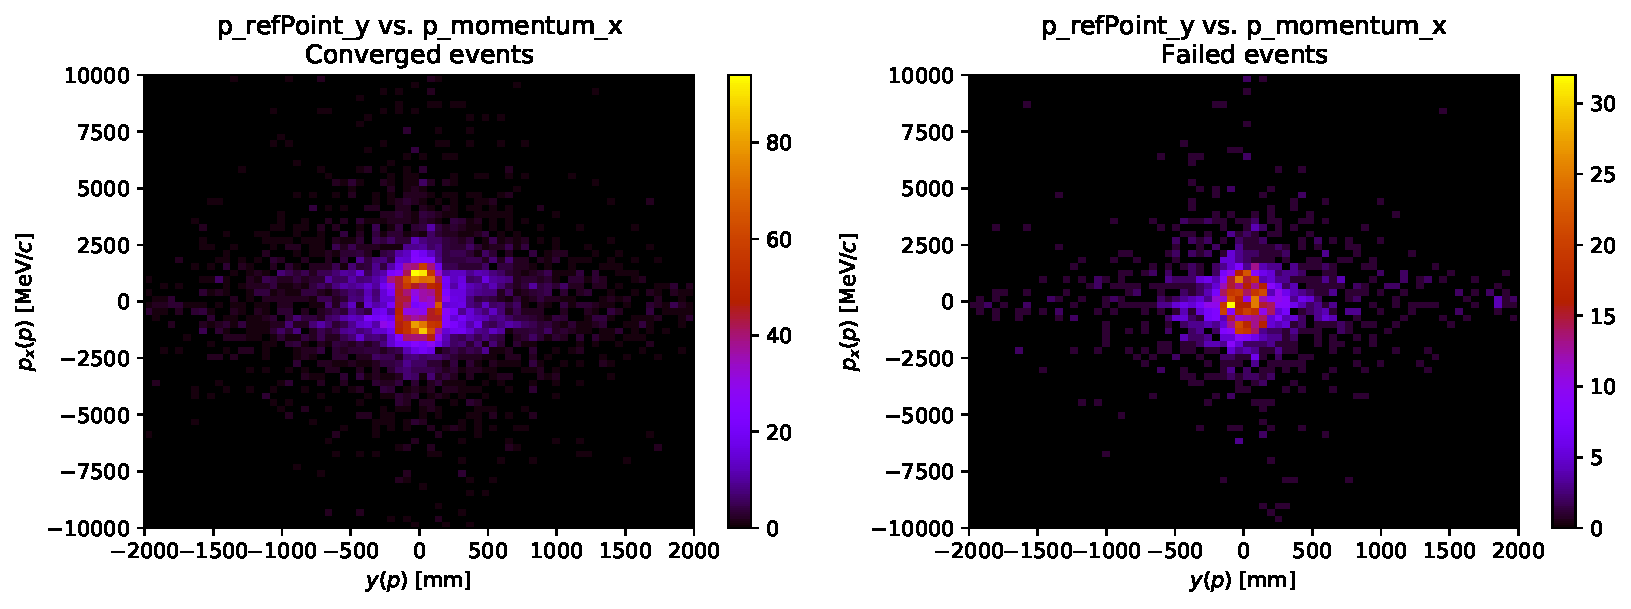
\includegraphics[width=\textwidth]{graphics/03-vertex_reconstruction/pp_p_refPoint_y_vs_p_momentum_x.pdf}
%	\caption{B.}
%	\label{fig:pp_p_px_vs_refpy_conv_vs_failed}
%\end{figure}
%
%Even more interestingly, this discrepancy can be put in relation to the $y$ component of the protoparticle first measurement position, as seen in Figure \ref{fig:pp_p_px_vs_refpy_conv_vs_failed}.
%The ring-like structure in Figure \ref{fig:pp_p_px_vs_refpy_conv_vs_failed} implies that the vertexing process struggles to reconstruct proton protoparticles with low $p_x$ hitting the T stations at $y\approx 0$.
%No such discrepancy is present in the case of pions.
%
%A precise estimate of $p_x$ is of paramount importance for correct track measurement and extrapolation.
%Even slight mistakes in angle assessment are magnified during particle transportation through long distances, especially since the T track requirement leaves no upstream constraints.
%Moreover, momentum itself is computed through evaluation of the particle bending curve in the $xz$ plane induced by the magnet.
%As such, it stands to reason that poor measurement of the low proton $p_x$ can have enough of an effect to throw off the vertexing algorithm.


\subsection{Decay kinematics after extrapolation}
\label{sec:3:true_vtx_kinematics}
As will be later discussed in Sections \ref{sec:blowup_matrix} and \ref{sec:lambda_endvertex_bias}, reconstruction of the \lz vertex is affected by a significant positive bias of median value $\mu_\frac{1}{2} \left(z_\Lambda^\text{reco} - z_\Lambda^\text{true}\right) \approx \SI{40}{\centi\meter}$.
In spite of such a discrepancy, the standard modus operandi for kine\-matics-at-vertex analyses usually compares true momenta (evaluated at the true vertex) with reconstructed momenta (evaluated at the reconstructed vertex), ignoring the discrepancy.

For this section I have followed a different approach, opting to transport via Runge-Kutta extrapolator the reconstructed $p$ and $\pi^-$ at the true $\Lambda^0 \rightarrow p\pi^-$ vertex position, injected from Monte Carlo information.
Tracks are transported to a given $z$ within extrapolator tolerance, leaving $x$ and $y$ coordinates (\textit{reference points}, henceforth) dependent on the initial measured momentum.

Since the extrapolator takes raw protoparticles as inputs, this process bypasses any smoothing applied during the fit process and, given an observable $f$ (particle reference points and momenta, for instance), it allows for a comparison between the true value $f_\text{true}$ and the RK-extrapolated value $f_\text{RK}$ at the actual $z_\text{vtx}^\Lambda$, circumventing the effect of vertex bias.
Any potential mismatch will be normalized in terms of \textit{pulls}
\begin{equation}
	\frac{f_\text{RK} - f_\text{true}}{\sigma_f^\text{RK}},
\end{equation}
with $\sigma_f^\text{RK}$ being the uncertainty computed by the RK extrapolator.
Assuming correct estimation of such uncertainties, we expect the pulls to follow a standard normal distribution.

\begin{figure}[t]
	\centering
	\begin{subfigure}{.45\textwidth}
		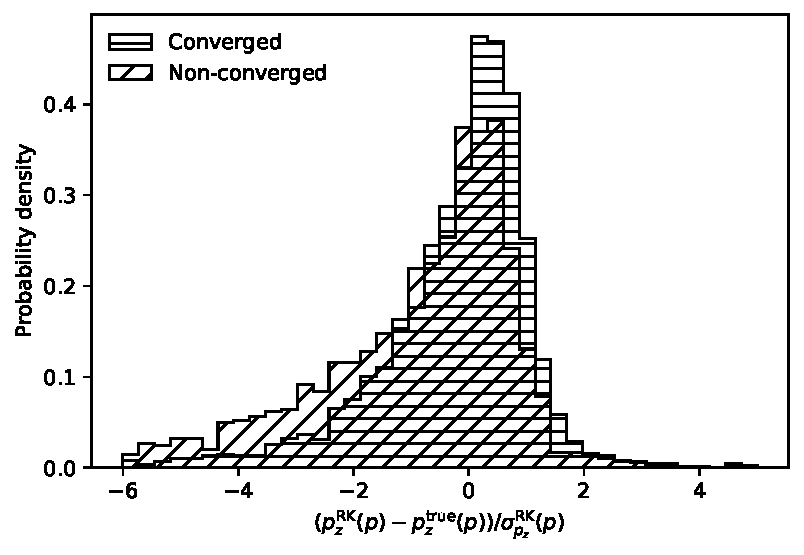
\includegraphics[width=\textwidth]{graphics/03-vertex_reconstruction/NONCONVERGED_p_momentum_residual_2Dv3D_z_rel.pdf}
		\caption{}
		\label{fig:p_momentum_residual_2Dv3D_z_rel}
	\end{subfigure}
	\begin{subfigure}{.45\textwidth}
		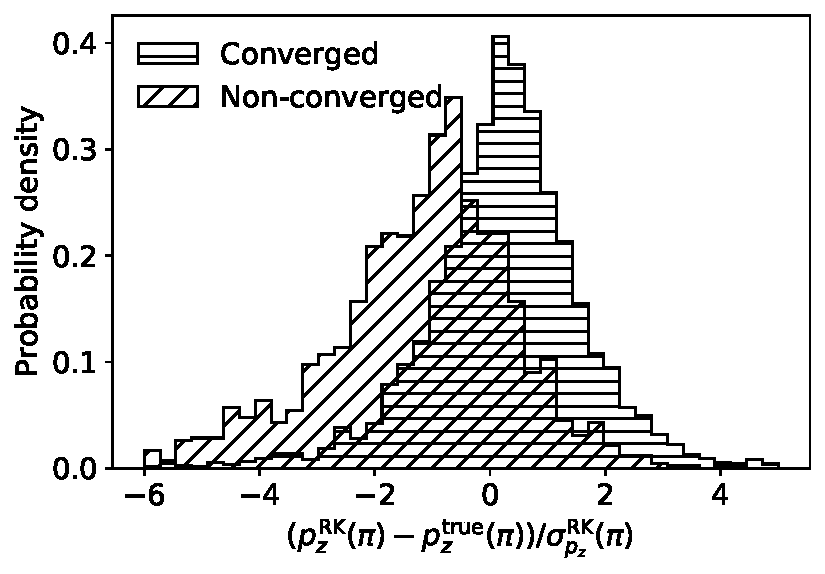
\includegraphics[width=\textwidth]{graphics/03-vertex_reconstruction/NONCONVERGED_pim_momentum_residual_2Dv3D_z_rel.pdf}
		\caption{}
		\label{fig:pim_momentum_residual_2Dv3D_z_rel}
	\end{subfigure}
	\caption{Normalized distributions of proton \textit{(a)} and pion \textit{(b)} $p_z$ pulls after track extrapolation at the true simulated \lambdadecay vertex. Distributions of events with converging vertex fit are depicted with \textit{horizontal hatching}, non-converging fit with \textit{diagonal hatching}.}
	\label{fig:p_pim_momentum_residual_2Dv3D_z_rel}
\end{figure}

Figure \ref{fig:p_pim_momentum_residual_2Dv3D_z_rel} shows $p_z$ pulls for proton and pions extrapolated at the \lz true decay vertex, juxtaposing converged and non-converged event distributions.
The first takeaway is that VF-reconstructed events have remarkably non-gaussian distributions, with slightly positive means and asymmetric tails. 
%This is particularly apparent in the case of the proton, where for $p_z^\text{RK} < p_z^\text{true}$ the RK algorithm systematically underestimates the error.
%More relevant for this chapter is
Moreover, Figure \ref{fig:pim_momentum_residual_2Dv3D_z_rel} highlights the fact that pion tracks from non-converged events generally sport a strong negative bias on $p_z$.

\begin{figure}[t]
	\centering
	\begin{subfigure}{.45\textwidth}
		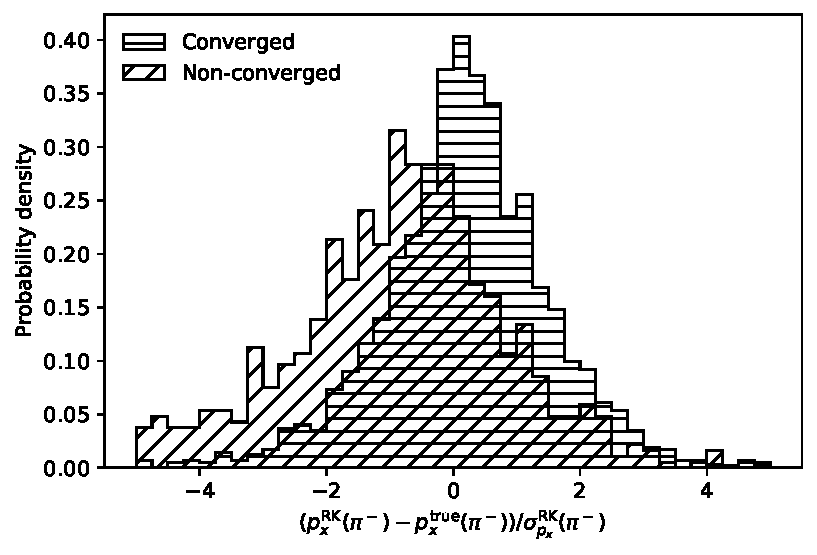
\includegraphics[width=\textwidth]{graphics/03-vertex_reconstruction/NONCONVERGED_pim_momentum_residual_2Dv3D_x_rel_matter.pdf}
		\caption{}
		\label{fig:pim_momentum_residual_2Dv3D_x_rel_matter}
	\end{subfigure}
	\begin{subfigure}{.45\textwidth}
		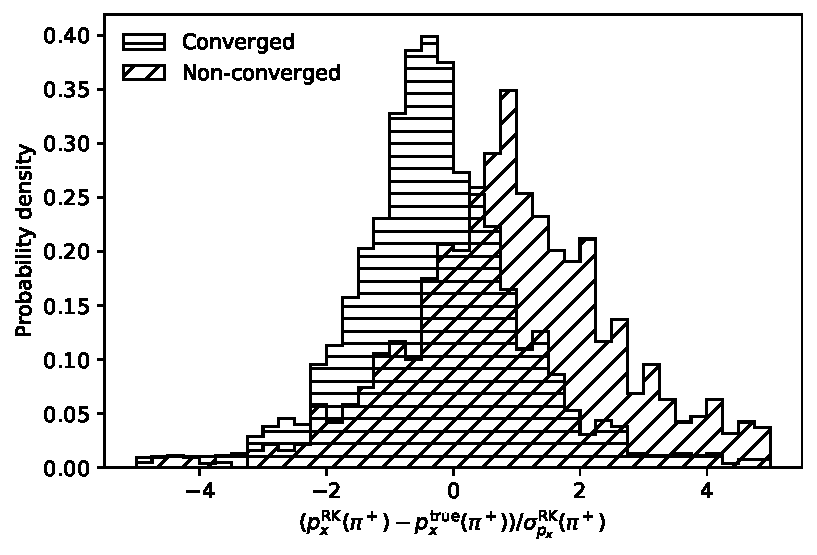
\includegraphics[width=\textwidth]{graphics/03-vertex_reconstruction/NONCONVERGED_pim_momentum_residual_2Dv3D_x_rel_antimatter.pdf}
		\caption{}
		\label{fig:pim_momentum_residual_2Dv3D_x_rel_antimatter}
	\end{subfigure}
	\caption{Normalized distributions of pion $p_x$ pulls in simulated $\Lambda^0 \rightarrow p\pi^-$ \textit{(a)} and $\bar{\Lambda}^0 \rightarrow \bar{p}\pi^+$ \textit{(b)} events after track extrapolation at the true $\Lambda^0$/$\bar{\Lambda}^0$ decay vertex.
	Distributions of events with converging vertex fit are depicted with \textit{horizontal hatching}, non-converging fit with \textit{diagonal hatching}.}
	\label{fig:3:pim_momentum_residual_2Dv3D_x_rel}
\end{figure}

Transverse momenta of proton and pions after transport show no similar biases when both $\Lambda^0 \rightarrow p\pi^-$ and $\bar{\Lambda}^0 \rightarrow \bar{p}\pi^+$ events are considered.
A significant bias in the extrapolated $p_x$ of both particles instead becomes visible when including only the former or latter class of events.
The situation for \lz decays is shown in Figure \ref{fig:pim_momentum_residual_2Dv3D_x_rel_matter}:
converged events bear a $leq 1\sigma$ positive $p_x$ bias for pions, while failed events are negatively biased with a much larger dispersion; the signs of both biases are reversed 
in $\bar{\Lambda}^0 \rightarrow \bar{p}\pi^+$ decays, as seen in Figure \ref{fig:pim_momentum_residual_2Dv3D_x_rel_antimatter}.

\begin{figure}[t]
	\centering
	\begin{subfigure}{.45\textwidth}
		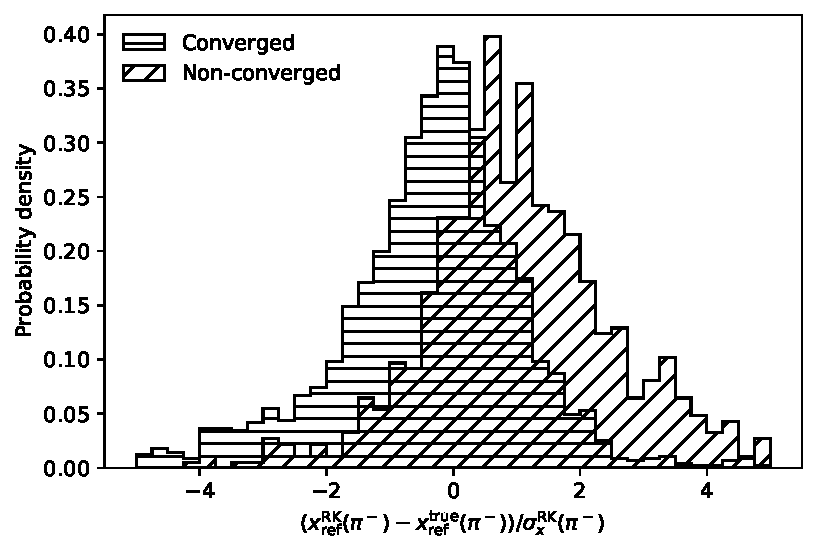
\includegraphics[width=\textwidth]{graphics/03-vertex_reconstruction/NONCONVERGED_pim_refpoint_residual_2Dv3D_x_rel_matter.pdf}
		\caption{}
		\label{fig:pim_refpoint_residual_2Dv3D_x_rel_matter}
	\end{subfigure}
	\begin{subfigure}{.45\textwidth}
		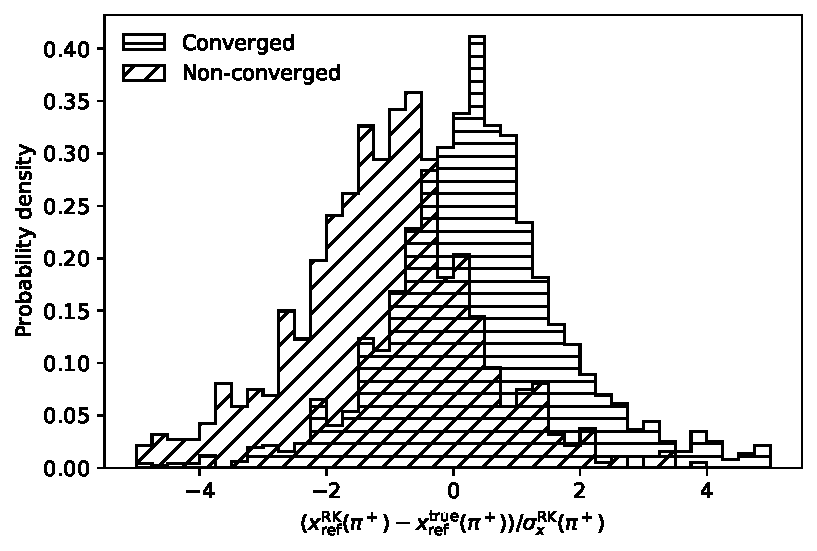
\includegraphics[width=\textwidth]{graphics/03-vertex_reconstruction/NONCONVERGED_pim_refpoint_residual_2Dv3D_x_rel_antimatter.pdf}
		\caption{}
		\label{fig:pim_refpoint_residual_2Dv3D_x_rel_antimatter}
	\end{subfigure}
	\caption{Normalized distributions of the $x$ component pulls of the pion reference point in simulated $\Lambda^0 \rightarrow p\pi^-$ \textit{(a)} and $\bar{\Lambda}^0 \rightarrow \bar{p}\pi^+$ \textit{(b)} events after track extrapolation at the true $\Lambda^0$/$\bar{\Lambda}^0$ decay vertex.
	Distributions of events with converging vertex fit are depicted with \textit{horizontal hatching}, non-converging fit with \textit{diagonal hatching}.}
	\label{fig:pim_refpoint_residual_2Dv3D_x_rel}
\end{figure}

This behaviour of the $p_x$ pulls also reflects on the $x$ components of the particle reference points after extrapolation, whose pulls are depicted in Figure \ref{fig:pim_refpoint_residual_2Dv3D_x_rel}.
For each class, $x_\text{ref}$ bias is opposite to the corresponding $p_x$ bias (e.g. $x_\text{ref}^\text{RK} > x_\text{ref}^\text{true}$ and $p_x^\text{RK} < p_x^\text{true}$ for pions in non-converging \lambdadecay events) and its sign flips when switching from matter to antimatter.

\begin{figure}[t]
	\centering	
	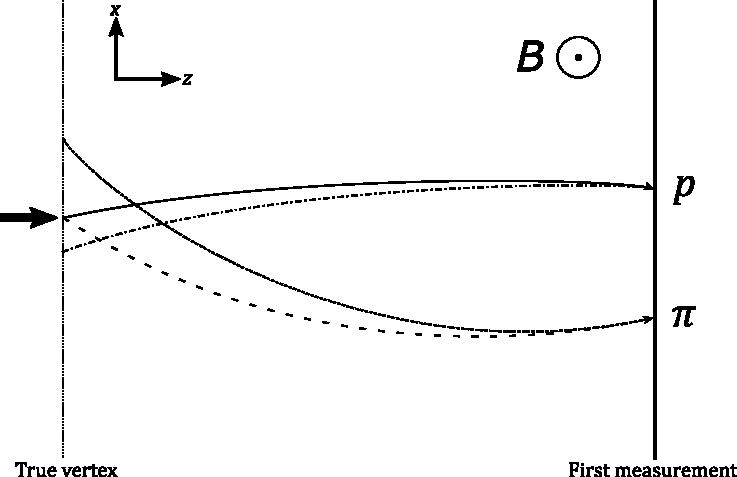
\includegraphics[width=.8\textwidth]{graphics/03-vertex_reconstruction/pim_bias_diagram_closing.pdf}
	\caption{Simplified \lambdadecay diagram demonstrating the relation between $p_z$ underestimation and bias on $\pi^-$ $x$ components of reference point and momentum after track extrapolation at the true vertex, denoted by the \textit{thick arrow on the left} and whose $z$ coordinate is traced with the \textit{vertical dotted line}.
	The true (extrapolated) proton track is drawn as a \textit{solid} (\textit{dash-dotted}) arrow, the pion as a \textit{dashed} (\textit{short-dashed}) arrow.
	The first measurement position, doubling as starting point for the backwards extrapolation, is marked by the \textit{thick vertical line on the right}.
	%The decay is shown in the $xz$ bending plane assuming the LHCb magnet in down polarity (this is equivalent to a $\bar{\Lambda}^0 \rightarrow \bar{p}\pi^+$ decay in up polarity).}
	The decay is shown in the $xz$ bending plane assuming the LHCb magnet in up polarity.}
	\label{fig:3:pion_biases_diagram}
\end{figure}

Bearing in mind that data for this analysis are simulated in magnet-up detector configuration, the discrepancies in $x_\text{ref}$ and $p_x$ pulls after extrapolation can be read as consequence of the $p_z$ systematic underestimation in non-converged decays seen in Figure \ref{fig:p_pim_momentum_residual_2Dv3D_z_rel}.
A particle's $p_z$ is intertwined with the bending curve imprinted by the magnetic field, as particles with higher $p_z$ will proportionally bend less (this is usually the case for protons, which carry most of the \lz momentum in its $p\pi^-$ decay).
The underestimation of $p_z$ thus results in overstated bending, and vice versa an overestimation of the bending curve during extrapolation will cause a lower $p_z$ at the true vertex;
this impacts in turn the $x$ component of the particle's reference point, introducing a bending-dependent offset with respect to the true vertex position.
This interpretation, illustrated in Figure \ref{fig:3:pion_biases_diagram} with a simplified diagram, links all three observed biases ($p_z$, $p_x$ and $x_\text{ref}$), explains the mirrored behaviour of \lz and $\bar{\Lambda}^0$ decays (bending direction is inverted due to opposite charge) and justifies the stronger impact on pions as opposed to protons, whose tracks are much more akin to straight lines due to higher average momentum.

%This behaviour can also be observed from a different perspective by considering the pion reference point $x$ residuals\footnote{}, plotted in Figure \ref{fig:pim_refpoint_residual_2Dv3D_x_rel}.
%For this part of the analysis, we forgo the established omission of charge-conjugate notation and separate events in matter ($\Lambda^0 \rightarrow p\pi^-$) and antimatter ($\bar{\Lambda}^0 \rightarrow \bar{p}\pi^+$) events.
%Since all events in this sample have magnet polarity $M_\text{pol} = +1$, i.e. magnetic field flowing towards the positive direction of the $y$ axis,
%%% @todo: controlla che sia vero
%matter and antimatter daughter particles will bend in opposite directions due to charge inversion.

%Comparing Figures \ref{fig:pim_refpoint_residual_2Dv3D_x_rel_matter} and \ref{fig:pim_refpoint_residual_2Dv3D_x_rel_antimatter}, $x$ components of pion reference points in non-converged events show opposite bias when extrapolated at the \lz vertex.
%Such a behaviour is easily understood in terms of transportation: tracks are extrapolated from downstream protoparticles towards decreasing $z$;
%if the magnetic bending effect in the $zx$ plane is overstated (if tracks <<bend too much>>), the resulting $x$ reference point at true $z_\text{vtx}^\Lambda$ will have an offset with respect to the actual origin vertex of the particle with polarity-dependdent sign (cf. Figure \ref{fig:zx_iter_failed}).

%Excessive bending is exactly what is expected of a track with correctly estimated $p_x$ and $p_y$, but underestimated $p_z$.
%Furthermore, a lower $p_z$ will affect the closest distance point between proton and pions in the $zx$ plane, but will have a much lower impact on the track crossing point in the $yz$ plane,
%%where bending is negligible,
%supporting the conflicting information interpretation for vertex oscillation given in Section \ref{sec:oscillation}.
Finally, the underestimation of pion $p_z$ is relevant to the problem of low vertex reconstruction efficiency.
The $xz$ and $yz$ propagation planes are affected differently by $p_z$ underestimation on account of the magnet bending in the former.
This can potentially result in the conflict between $xz$ and $yz$ topologies observed in non-converged events, the current leading hypothesis to explain the oscillatory behaviour of the VF algorithm which prevents decay convergence.
Considering the information gathered so far,
the most plausible cause of this $p_z$ bias appears to be poor momentum measurement at T station level.
%While wrong extrapolation by the Runge-Kutta algorithm was considered as a possible source of bias...
%the two most plausible causes of this $p_z$ bias appear to be wrong extrapolation by the Runge-Kutta algorithm, perhaps triggered by lower protoparticle $p_x$ observed in Section \ref{sec:3:kinematics_at_first_meas}, and/or poor measurement from T stations resulting in $p_z$ underestimation of protons and pions.


%\section{Recovery of non-converged events}
%\subsection{Recovery through refit with rescaled uncertainties}
\section[Recovery of non-converged events]{Recovery of non-converged events through refit with rescaled uncertainties}
\label{sec:recovery_general}
\label{sec:blowup_matrix}

%\subsection{Recovery through interpolation}
%@todo

%\begin{figure}[t]
%	\centering
%	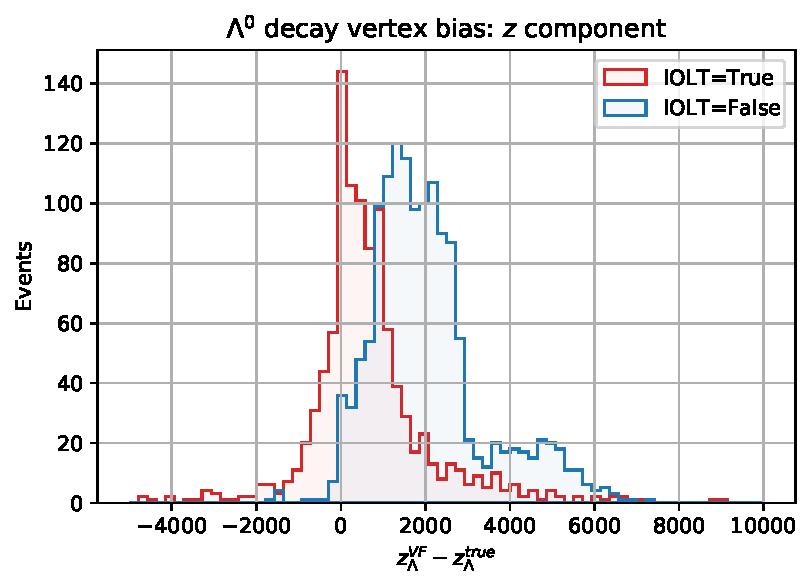
\includegraphics[width=.6\textwidth]{graphics/03-vertex_reconstruction/iolt_lambda_endvertex_z_bias.pdf}
%	\caption{A.}
%\end{figure}

As outlined in Section \ref{sec:oscillation}, vertexing failures in the $\Lambda^0 \rightarrow p\pi^-$ decay can be attributed to candidate vertices in different planes providing conflicting information.
To circumvent this phenomenon, my proposal for the recovery of these failed events involves performing an additional fit of the vertex (also referred to as \textit{refit} in the following pages) with a slightly altered version of the standard Vertex Fitter algorithm designed to attribute greater importance to a specific propagation plane.

The reasonable choice for this plane would be the $yz$ plane, since extrapolation of tracks does not need to be concerned with magnet bending and is therefore expected to be less prone to error.
However, this would penalize events with poor $yz$ protoparticle reconstruction, for instance events with parallel or diverging tracks in said plane.
To maximize the recovery efficiency of my solution, I have elected to perform three separate refits on non-converging events, prioritizing $yz \rightarrow xz \rightarrow xy$ planes in this order.
In a worst-case scenario, this would quadruple the time complexity of the vertexing process; in practice, half of all events converge with the standard VF, and about $\approx 15\%$ more converge after the first refit attempt ($yz$ plane).
%%@todo: stima dell'aumento del tempo

Considering the $yz$ plane as an example, we can prioritize available track information in this plane by artificially increasing the uncertainty $\sigma_x$ of the $x$ component of the candidate vertex position $\vec{x}$.
At each step in a VF iteration, $\vec{x}$ is updated according to \eqref{eq:VF_new_vertex_final}.
Uncertainties enter the computation through three terms:
\begin{enumerate}
	\item ${(C_{k-1}^i)}^{-1}$, the inverse vertex covariance matrix computed at the previous step (or final step of the previous iteration);
	\item ${(G_k^i)}_r$, the inverse covariance matrix of reference point $\vec{r}_k^i$, computed at the true transport of particle $k$;
	\item $C_k^i$, the current vertex covariance matrix, inverted from the matrix sum of the previous two terms as in \eqref{eq:3:VF_new_inv_covmatrix}.
\end{enumerate}
Ergo, the best approach to increase $\sigma_x$ while minimizing additional computation time is to act on the individual components of ${(C_{k-1}^i)}^{-1}$ and ${(G_k^i)}_r$ just before the \eqref{eq:3:VF_new_inv_covmatrix} sum.

Assuming gaussian uncertainties, a standard three-dimensional covariance matrix will have the form
\begin{equation}
C = \begin{pmatrix}
	\sigma_x^2 & \rho_{xy} \sigma_x \sigma_y & \rho_{xz} \sigma_x \sigma_z \\
	\rho_{xy} \sigma_x \sigma_y & \sigma_y^2 & \rho_{yz} \sigma_y \sigma_z \\
	\rho_{xz} \sigma_x \sigma_z & \rho_{yz} \sigma_y \sigma_z & \sigma_z^2 \\
\end{pmatrix},
\label{eq:3:gaussian_covmatrix}
\end{equation}
where $\rho_{ij} \coloneqq \text{corr}(i,j)$. Its inverse matrix is written as
\begin{equation}
C^{-1} = \frac{1}{K} \begin{pmatrix}
%%%%%%%%%%%%%%%%%%%%%%%%%%%%%%%%%%%
\frac{1-\rho_{yz}^2}{\sigma_x^2} &&
\frac{\rho_{xz}\rho_{yz} - \rho_{xy}}{\sigma_x \sigma_y} &&
\frac{\rho_{xy}\rho_{yz} - \rho_{xz}}{\sigma_x \sigma_z} \\
%%%%%%%%%%%%%%%%%%%%%%%%%%%%%%%%%%%
\frac{\rho_{xz}\rho_{yz} - \rho_{xy}}{\sigma_x \sigma_y} &&
\frac{1-\rho_{xz}^2}{\sigma_y^2} &&
\frac{\rho_{xy}\rho_{xz} - \rho_{yz}}{\sigma_y \sigma_z} \\
%%%%%%%%%%%%%%%%%%%%%%%%%%%%%%%%%%%
\frac{\rho_{xy}\rho_{yz} - \rho_{xz}}{\sigma_x \sigma_z} &&
\frac{\rho_{xy}\rho_{xz} - \rho_{yz}}{\sigma_y \sigma_z} &&
\frac{1-\rho_{xy}^2}{\sigma_z^2}
\end{pmatrix},
\label{eq:3:inverse_gaussian_covmatrix}
\end{equation}
with
\begin{equation}
K \coloneqq \frac{\det C}{\sigma_x^2 \sigma_y^2 \sigma_z^2} = 1+2\rho_{xy} \rho_{xz} \rho_{yz} - \rho_{xy}^2 - \rho_{xz}^2 - \rho_{yz}^2.
\end{equation}
Going back to the $yz$ plane example, we increase $\sigma_x$ by introducing a multiplicative factor $s_x < 1$ for relevant covariance matrix components as follows:
\begin{equation}
\begin{aligned}
&C^{-1}_{xx} = C^{-1}_{xx} \times s_x^2, \\
&C^{-1}_{xy} = C^{-1}_{yx} = C^{-1}_{xy} \times s_x, \\
&C^{-1}_{xz} = C^{-1}_{zx} = C^{-1}_{xz} \times s_x,
\end{aligned}
\label{eq:3:sigma_x_rescaled}
\end{equation}
with other components left as is.
This process is also applied to ${(G_k^i)}_r$ and replicated at each step of the refit algorithm, which I'll refer to as \textit{$\sigma_x$-rescaled}.
Similarly, the $\sigma_y$-rescaled and $\sigma_z$-rescaled algorithms prioritize planes $xz$ and $xy$ respectively (their extension from \eqref{eq:3:sigma_x_rescaled} is trivial).
For the remainder of this section, I'll refer to their sequential application $\sigma_x \rightarrow \sigma_y \rightarrow \sigma_z$ as the \textit{$\sigma$-rescaled refit process}.

As proof of concept, I have analyzed the performance of the $\sigma$-rescaled refit approach on the sample of 110\,000 MC-generated \demonstratorshort events previously used in this chapter.
Choosing $s_i=0.98, i\in\{x,y,z\}$, which maximizes the number of events recovered by the refit and corresponds to a $\approx 2\%$ increase in vertex uncertainties, I observed a $+26.4\%$ increase in reconstructed signal.
Given a vertexing efficiency $\lesssim 50\%$, as reported in Figure \ref{fig:lambda_lambdab_reco_efficiency}, this amounts to roughly a quarter of all missing reconstructible decays.
Within these recovered events, 57.1\% converge under the $\sigma_x$ algorithm, 38.1\% under the $\sigma_y$ algorithm and the remaining 4.8\% under the $\sigma_z$ algorithm.

%% Nota: non c'è colonna per i valori su tutti gli eventi ricostruiti con il tale algoritmo perché perlopiù sono inseriti nella tabella precedente.
%% Nota: i valori nell'altra tabella sono molto più alti perché escludono i VF!!
\begin{table}[t]
	\begin{center}
	\begin{tabular}{@{}lllllll@{}}
		\toprule
		Algorithm & \multicolumn{6}{c}{Median $\tilde{\chi}^2_\text{vtx}(\Lambda^0)$} \\
		\cmidrule{2-7}
		& Common events & Exclusive events & \multicolumn{4}{c}{Pair-shared events}  \\
		\cmidrule{4-7}
		&&& VF & $\sigma_x$ & $\sigma_y$ & $\sigma_z$ \\
		\midrule
		VF 			& 1.35 & 0.32	& --	& 1.06	& 1.28	& 1.36	 \\
		$\sigma_x$ 	& 1.36 & 3.18	& 1.09	& --	& 1.61	& 1.84	 \\
		$\sigma_y$	& 1.38 & 3.13	& 1.32	& 1.63	& -- 	& 1.96	 \\
		$\sigma_z$ 	& 1.41 & 51.52	& 1.45	& 1.88	& 2.01	& --	 \\
		\bottomrule
	\end{tabular}
	\end{center}
	\caption{Comparison of median $\tilde{\chi}^2_\text{vtx}$ of the \lambdadecay vertex fit performed by the Vertex Fitter and the three $\sigma$-rescaled algorithms. Performances are reported on common events reconstructed by all four algorithms, on exclusive events reconstructed only by a specific algorithm, and on events reconstructed pairwise by at least two algorithms.}
	\label{tab:3:xyz_chi2_performances}
\end{table}

I have also run each individual $\sigma$-rescaled algorithm in isolation (without the Vertex Fitter) on the simulated signal to evaluate their performances on all events, including standard-converging ones.
Before proceeding, a digression is in order to better understand the meaning of \textit{performance} when comparing the algorithms.
Table \ref{tab:3:xyz_chi2_performances} shows the median $\chi^2_\text{vtx}$ of the reconstructed vertices on specific subsamples of events:
\begin{itemize}
	\item \textit{common} events converging under Vertex Fitter and all three $\sigma$-rescaled algorithms;
	\item \textit{pairwise shared} events converging under (at least) two algorithms (e.g. VF and $\sigma_x$-rescaled, including events that may also converge under $\sigma_y$-rescaled);
	 \item \textit{exclusive} events only reconstructed by one particular algorithm.
\end{itemize}
%First I considered \textit{common} events, i.e. events converging under Vertex Fitter and all three $\sigma$-rescaled algorithms;
For common events, algorithm performances show very little variation, with a marginal performance hierarchy of $\text{VF} > \sigma_x > \sigma_y > \sigma_z$.
The aforementioned hierarchy also holds in pairwise shared events:
for instance, VF-$\sigma_x$ events have VF vertices with median $\tilde{\chi}^2_\text{vtx}$ of 1.06, slightly lower than the 1.09 of $\sigma_x$ vertices.

\begin{figure}[t]
	\centering
	\begin{subfigure}{.45\textwidth}
		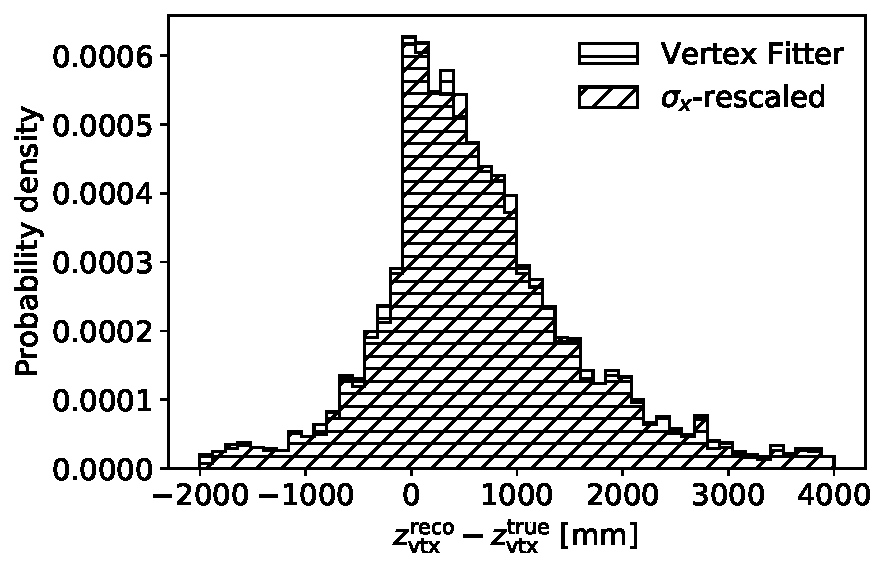
\includegraphics[width=\textwidth]{graphics/03-vertex_reconstruction/VF_vs_2DX_Lambda_endvertex_z_bias_common.pdf}
		\caption{}
		\label{fig:3:3D_vs_2D_lambda_endvertex_bias_common}
	\end{subfigure}
	\begin{subfigure}{.45\textwidth}
		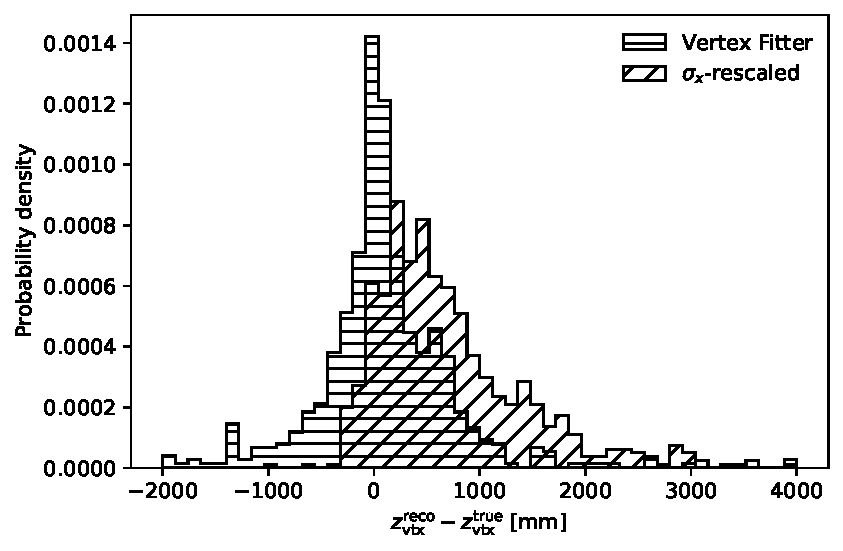
\includegraphics[width=\textwidth]{graphics/03-vertex_reconstruction/VF_vs_2DX_Lambda_endvertex_z_bias_exclusive.pdf}
		\caption{}
		\label{fig:3:3D_vs_2D_lambda_endvertex_bias_exclusive}
	\end{subfigure}
	\caption{Normalized distributions of bias on the \lambdadecay vertex $z$ component reconstructed by the standard Vertex Fitter (\textit{horizontal hatching}) and $\sigma_x$-rescaled (\textit{diagonal hatching}) algorithms. The algorithms were individually run on the same simulated \demonstratorshort sample: \textit{(a)} shows distributions for events reconstructed by both algorithms, \textit{(b)} shows distributions for events only reconstructed by one or the other.}
	\label{fig:3:3D_vs_2D_lambda_endvertex_bias_common_vs_exclusive}
\end{figure}

Where algorithm performances truly diverge is in exclusive events.
Events only converging under VF have a median $\tilde{\chi}^2_\text{vtx}$ of 0.32, while both $\sigma_x$ and $\sigma_y$ hover around a subpar $\approx 3$ and the $\sigma_z$ algorithm reaches an off-scale value of 51.
This discrepancy is also seen from a different perspective in Figure \ref{fig:3:3D_vs_2D_lambda_endvertex_bias_common_vs_exclusive}: the $z_\text{vtx}^\Lambda$ residual distributions for VF and $\sigma_x$-rescaled algorithms on shared events are indistinguishable (Figure \ref{fig:3:3D_vs_2D_lambda_endvertex_bias_common}), while $\sigma_x$-exclusive events have a significant positive bias compared to the unbiased VF-exclusive ones (Figure \ref{fig:3:3D_vs_2D_lambda_endvertex_bias_exclusive}).
This means that, while a minor hierarchy in fit quality does exist in the $\sigma$-rescaled algorithms, justifying the selected $\sigma_x \rightarrow \sigma_y \rightarrow \sigma_z$ refit order, large discrepancies in performances are due to the specific events reaching convergence under a specific algorithm.
%The reason for the high median $\tilde{\chi}^2_\text{vtx}$ in $\sigma_z$-exclusive \lambdadecay decays is to be searched in poor track information in $xz$ and $yz$ planes, preventing convergence with $\sigma_x$/$\sigma_y$ algorithms and resulting in mediocre fits, rather than in a fault of the $\sigma_z$-rescaled implementation.
The most likely explanation for the diminishing fit quality in $\sigma$-rescaled algorithms is poor track information in the relevant propagation planes:
for instance, an event only converging with the $\sigma_z$-rescaled algorithm must have subpar information in the $xz$ and $yz$ planes (preventing convergence with VF, $\sigma_x$- and $\sigma_y$-rescaled algorithms), and favouring information in the $xy$ plane when deciding the best vertex will lead to poor resolution in $z_\text{vtx}^\Lambda$.
This interpretation also explains the large fit quality gap between exclusive $\sigma_x$- and $\sigma_y$-converging events ($\tilde{\chi}^2_\text{vtx} (\Lambda^0) \approx 3$) and exclusive $\sigma_z$-converging events ($\tilde{\chi}^2_\text{vtx} (\Lambda^0) \approx 51$), as the latter algorithm forgoes most information for the crucial $z$ axis.

\begin{table}[t]
	\begin{center}
	\begin{tabular}{@{}lllll@{}}
		\toprule
		Algorithm & Statistics increase & Median $\tilde{\chi}^2_\text{vtx}(\Lambda^0)$ & \multicolumn{2}{c}{Median bias} \\
		\cmidrule{4-5}
		&&& $z_\text{vtx}^\Lambda$ [mm] & $p_z^\text{DTF} (p)$ \\
		\midrule
		VF  	 	& -- 		& 1.0 	& 399 & $+0.02\%$	\\
		\midrule
		$\sigma_x$ 	& $+15.0\%$	& 6.1 	& 541 & $-0.48\%$ 	\\
		$\sigma_y$ 	& $+18.9\%$	& 5.8	& 573 & $-1.12\%$ 	\\
		$\sigma_z$ 	& $+20.7\%$	& 9.2 	& 729 & $-0.71\%$  	\\
		Sequential 	& $+26.4\%$	& 7.1 	& 604 & $-0.81\%$ 	\\
		\bottomrule
	\end{tabular}
	\end{center}
	\caption{Performance comparison of the three $\sigma$-rescaled algorithms with $s_i=0.98$, their sequential application ($\sigma_x \rightarrow \sigma_y \rightarrow \sigma_z$) and the standard Vertex Fitter algorithm.
	%Recovery efficiency for each $\sigma$-rescaled algorithm is computed over the total number of events recovered by their sequential application.
	%Median performances for $\sigma_i$-rescaled algorithms are computed on all events recovered with the algorithm, including events also reaching convergence with other $\sigma$-rescaled algorithms, while values for the Vertex Fitter are computed on standard reconstructed events.
	Median values for shown variables are computed on recovered events for $\sigma$-rescaled algorithm, standard reconstructed events for the Vertex Fitter.
	Proton $p_z$ is computed using the Decay Tree Fitter algortihm with \jpsi and \lz mass constraints.}
	\label{tab:3:xyz_VF_performances}
\end{table}

\begin{figure}[t]
	\centering
	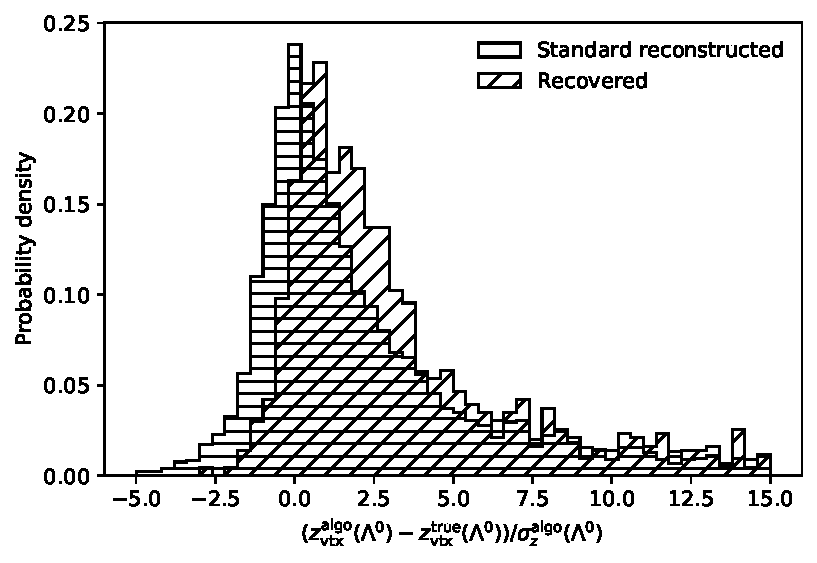
\includegraphics[width=.6\textwidth]{graphics/03-vertex_reconstruction/Lambda_endvertex_z_bias_pulls_2D_vs_3D.pdf}
	\caption{Normalized distribution of $z_\text{vtx}^\Lambda$ pulls in simulated \demonstratorshort events: decays reconstructed with the Vertex Fitter are labeled with \textit{horizontal hatching}, decays recovered via the sequential application of $\sigma$-rescaled algorithms with \textit{diagonal hatching}.}
	\label{fig:3:xyz_L_ENDVERTEX_residual_2Dv3D_z_rel}
\end{figure}

With this in mind, Table \ref{tab:3:xyz_VF_performances} reports the performance of the three $\sigma$-rescaled algorithms and the full $\sigma$-rescaled refit process on recovered events, compared to the VF performance on standard reconstructed events.
The overall $\tilde{\chi}^2_\text{vtx}$ of the \lambdadecay vertex for recovered events is significantly worse than the expected 1.0 value obtained by the VF;
likewise, the median $\approx \SI{40}{\centi\meter}$ $z_\text{vtx}^\Lambda$ bias in VF events (discussed more in detail in Section \ref{sec:lambda_endvertex_bias}) is still \SI{20}{\centi\meter} lower than in recovered events (also shown in terms of pulls in Figure \ref{fig:3:xyz_L_ENDVERTEX_residual_2Dv3D_z_rel}).
As discussed in Section \ref{sec:3:true_vtx_kinematics}, non-converging events show a systematic $p_z$ underestimation in pion T tracks, which also reflects on recovered events in the negative $p_z$ bias computed with the Decay Tree Fitter algorithm using \jpsi and \lz mass constraints (Table \ref{tab:3:xyz_VF_performances}).
This phenomenon explains the increased $z_\text{vtx}^\Lambda$ bias, as a lower $p_z$ at T station position translates in an apparent crossing point downstream of the actual vertex (this is exemplified in Figure \ref{fig:3:pion_biases_diagram}).

%This increased bias is an anticipated consequence of the systematic T track $p_z$ underestimation discussed in , which also reflects in the negative $p_z$ bias computed by the Decay Tree Fitter algorithm with \jpsi and \lz mass constraints on recovered events.

Tables \ref{tab:3:xyz_chi2_performances} and \ref{tab:3:xyz_VF_performances} confirm that the $\sigma_z$-rescaled algorithm is by far the worse performing of the three.
This is a somewhat expected consequence of partially forgoing $xz$ and $yz$ information in the fit, and placing this algorithm last in the process ensures that it only affects events which would not converge under other circumstances.
In the context of the proof-of-concept study, I elected to include the $\sigma_z$-rescaled algorithm in the refit process to gain a more complete view of its capabilities.
However, were the ensuing events to be considered too poorly reconstructed for the \lz analysis, the algorithm could feasibly be omitted ss it only contributes a negligible $+1.3\%$ of additional signal.

In conclusion, my $\sigma$-rescaled refit process allows for a $+26.4\%$ increase in reconstructed signal events.
While $\tilde{\chi}^2_\text{vtx}$ and bias on $z_\text{vtx}^\Lambda$ are higher compared to events reconstructed via Vertex Fitter, there is sufficient evidence pointing towards this being a problem intrinsic to the non-converged events themselves.
Because of the timing requirements to perform a re-reconstruction of the full data sample (described in Section \ref{sec:2:used_data}), I didn't employ recovered events for the remainder of the analysis.
The impact of their increased bias on the prospective \lz EDM/MDM measurement will have to be evaluated in dedicated sensitivity studies and possibly incorporated as a source of systematic uncertainty to be accounted for.


%%%%%%%%%%%%%%%%%%%%%%%%%%%%%%%%%%%%%%% Questa parte è da riscrivere, my boy. Devi mettere in chiaro che non è "poor performance", è che fanno schifo gli eventi.
%In terms of recovery power, the $\sigma_z$-rescaled algorithm favouring $xy$ plane information is the best one, providing a $+20.7\%$ increase in statistics when run in isolation.
%Unfortunately, said algorithm also contributes 

%%%%%%%%%%%%%%%%%%%%%%%%%%%%

%I have also run each algorithm individually after the standard VF to gauge their performance on the $n^\text{reco}_\text{tot}$ recovered events.
%Results of this test are compiled in Table \ref{tab:3:xyz_VF_performances}.
%When considering the \textit{recovery efficiency} of each algorithm, defined as the fraction of recovered events converging under said algorithm, i.e.
%\begin{equation}
%	\varepsilon^\text{reco}_i \rvert_{i\in\{x,y,z\}} = \frac{n_i^\text{reco}}{n_\text{tot}^\text{reco}},
%\end{equation}
%the $\sigma_z$-rescaled is the better performing one, reaching convergence in $\approx 80\%$ of recoverable events.
%Despite this, all three $\sigma$-rescaled algorithms have a sizable number of <<exclusive>> events that do not reach convergence under any other variation.
%Furthermore, while the $\sigma_z$-rescaled does recover more events by itself, only $\approx 5\%$ of the total recovered events are exclusive to it, meaning its overall impact on the $\sigma$-rescaled refit process is low.

%The established $\sigma_x \rightarrow \sigma_y \rightarrow \sigma_z$ refit order is justified in light of performance evaluation based on the goodness of these fits.
%As seen again in Table \ref{tab:3:xyz_VF_performances}, the $\sigma_x$-rescaled algorithm has comparatively lower vertex $\tilde{\chi}^2$, $z_\text{vtx}^\Lambda$ bias and proton $p_z$ bias using the DTF algorithm with \jpsi and \lz mass constraints.
%Using the $\sigma_z$-rescaled algorithm as last resort means only $\approx 5\%$ of recovered events are actually affected by its poor performance.

%\begin{figure}[t]
%	\centering
%	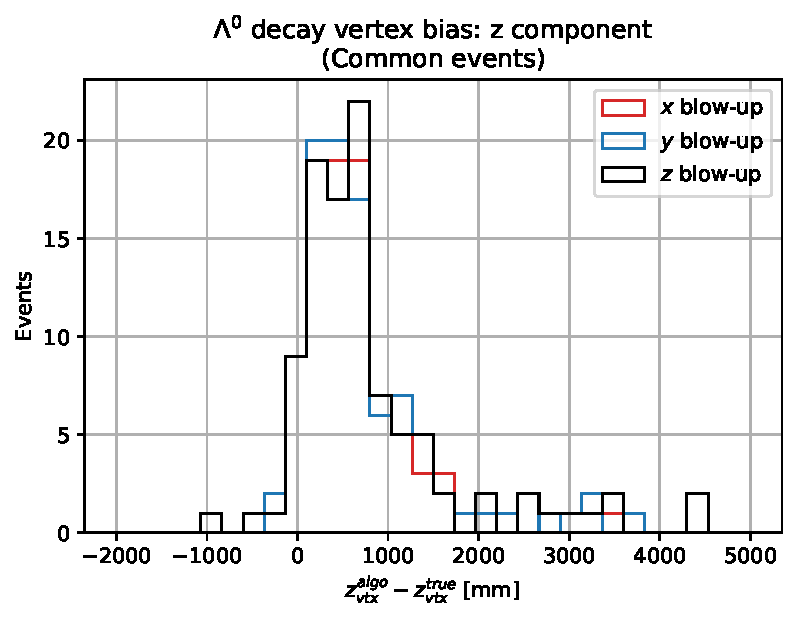
\includegraphics[width=.6\textwidth]{graphics/03-vertex_reconstruction/Lambda_endvertex_z_bias_xyz_common.pdf}
%	\caption{A.}
%	\label{fig:3:Lambda_endvertex_z_bias_xyz_common}
%\end{figure}
%
%Figure \ref{fig:3:Lambda_endvertex_z_bias_xyz_common} shows the $z_\text{vtx}^\Lambda$ bias of the individual $\sigma$-rescaled algorithms in the $\approx 36\%$ of recovered events which converge under all three variations.
%Despite the difference in performance outlined in Table \ref{tab:3:xyz_VF_performances}

%All $\sigma$-rescaled algorithms still appear to perform significantly worse than the standard VF on all the above fronts.
%To investigate this, I have individually run the $\sigma_x$-rescaled and standard VF algorithms on all available events and compared their results.
%Considering the total number of events reconstructed by combining the two, $\approx 74\%$ of them are reconstructed by both, $\approx 13\%$ are only reconstructed by the $\sigma_x$-rescaled (these are the $\sigma_x$-recovered events from Table \ref{tab:3:xyz_VF_performances}) and a roughly equal $\approx 13\%$ of them are only reconstructed by the Vertex Fitter.
%
%What's more interesting is the performance comparison. Figure \ref{fig:3:3D_vs_2D_lambda_endvertex_bias_common} shows the $z_\text{vtx}^\Lambda$ bias on events common to VF and $\sigma_x$-rescaled.
%Despite the median \SI{15}{\centi\meter} discrepancy reported in Table \ref{tab:3:xyz_VF_performances}, the two distributions are indistinguishable from the other.
%The expected difference only emerges when considering events exclusive to each algorithm, as seen in Figure \ref{fig:3:3D_vs_2D_lambda_endvertex_bias_exclusive}.

%The differences in $z_\text{vtx}^\Lambda$ and proton $p_z^\text{DTF}$ bias are therefore to be understood in terms of what events reach convergence with a specific algorithm, rather than as performance evaluations of the algorithm itself.
%The $\sigma_x$-rescaled algorithm does not intrinsically reconstruct events with larger bias;
%instead, its $yz$-centric approach allows it to recover events that throw off the standard VF, and these events tend to have a larger $z_\text{vtx}^\Lambda$ bias on their best vertex candidate.
%This tendency is likely the result of the systematic T track $p_z$ underestimation analyzed in Section \ref{sec:3:kinematics_at_first_meas}.

%%@todo: se trovi un posto adatto, menziona che xyz insieme non fungono. Non è che sia importante.

\section{\texorpdfstring{\lz}{Lambda} decay vertex bias in standard reconstructed events}
\label{sec:lambda_endvertex_bias}

So far I have focused on the additional bias on $z_\text{vtx}^\Lambda$ introduced by the newly recovered events.
As previously remarked, however, standard reconstructed events are significantly biased as well.
The quality of the \lambdadecay vertex reconstruction affects many aspects of the $\Lambda^0$ electromagnetic dipole moments measurement outlined in Section \ref{sec:lambda}:
on top of being fundamental to evaluate how much magnetic field the particle traversed (and thus the extent of spin precession), even the best momentum resolution for protons and pions is worthless if the particles are extrapolated at the wrong point of production.
This section will therefore focus on biases in \lambdadecay vertexing affecting already reconstructed events.
Since both $x_\text{vtx}^\Lambda$ and $y_\text{vtx}^\Lambda$ are fairly well reconstructed, with resolution $\lesssim \SI{1}{\centi\meter}$ and no discernible bias, the focus will be on the reconstruction of $z_\text{vtx}^\Lambda$.
The following results are obtained from the complete simulated \demonstratorshort dataset (see Section \ref{sec:2:used_data}) after the full selection process detailed in Chapter \ref{cap:event_selection}, unless otherwise specified.

%\begin{figure}[t]
%	\centering
%	\begin{subfigure}{.45\textwidth}
%		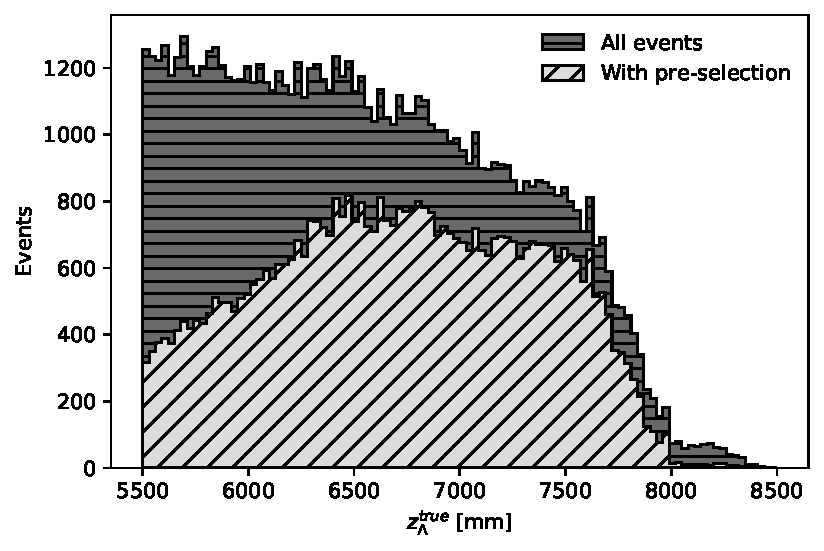
\includegraphics[height=.2\textheight]{graphics/04-event_selection/Lambda_endvertex_z_true.pdf}
%		\caption{}
%		\label{fig:4:lz_vertex_true}
%	\end{subfigure}
%	\begin{subfigure}{.45\textwidth}
%		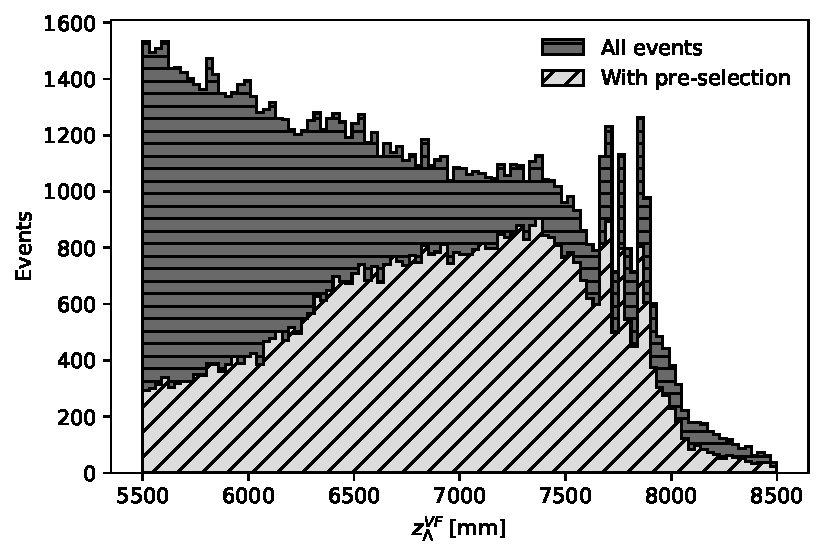
\includegraphics[height=.2\textheight]{graphics/04-event_selection/Lambda_endvertex_z.pdf}
%		\caption{}
%		\label{fig:4:lz_vertex_reco}
%	\end{subfigure}
%	\caption{Distribution of true \textit{(a)} and reconstructed \textit{(b)} $z_\text{vtx}^\Lambda$ in simulated \demonstratorshort signal events, without (\textit{dark grey}) and with (\textit{light grey}) prefiltering.}
%	\label{fig:4:lz_vertex_distributions}
%\end{figure}
%
%\begin{figure}[t]
%	\centering
%	\begin{subfigure}{.45\textwidth}
%		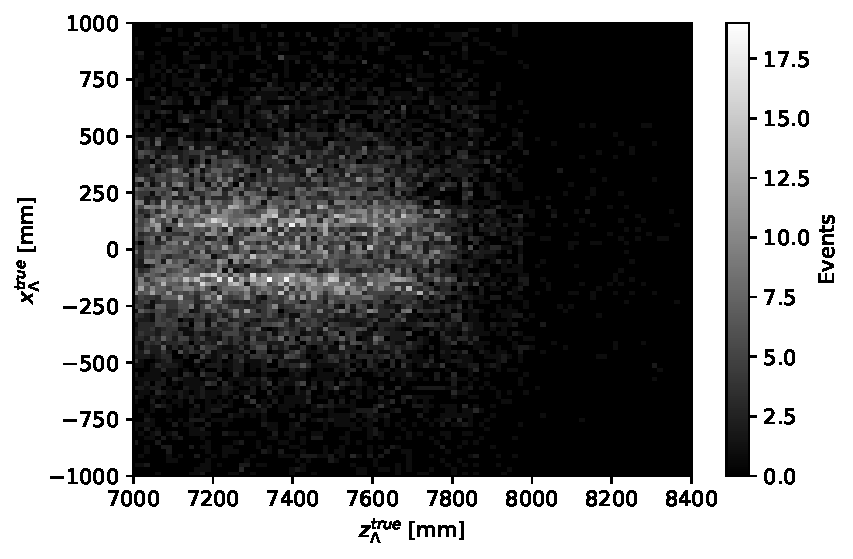
\includegraphics[height=.2\textheight]{graphics/04-event_selection/Lambda_endvertex_z_vs_x_true.pdf}
%		\caption{}
%		\label{fig:4:lz_vertex_peaks_true}
%	\end{subfigure}
%	\begin{subfigure}{.45\textwidth}
%		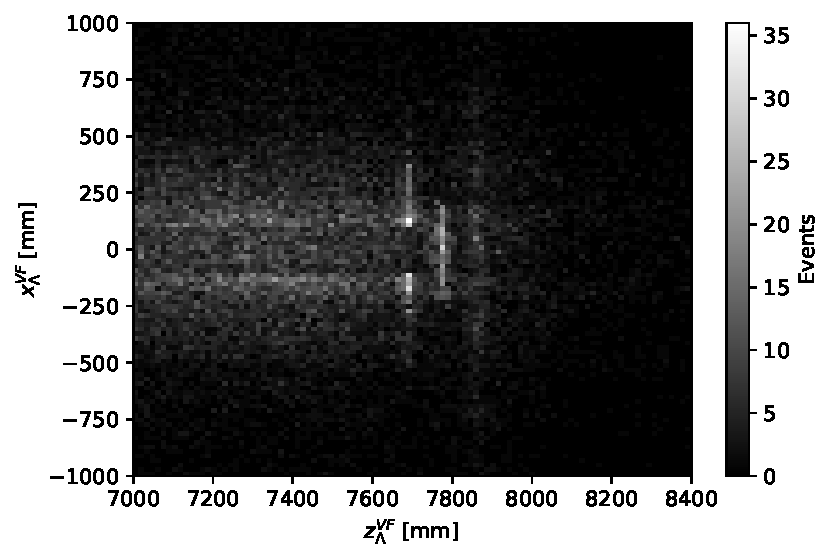
\includegraphics[height=.2\textheight]{graphics/04-event_selection/Lambda_endvertex_z_vs_x.pdf}
%		\caption{}
%		\label{fig:4:lz_vertex_peaks_reco}
%	\end{subfigure}
%	\caption{Distribution of simulated \demonstratorshort signal events (prefilters applied) with $z_\Lambda^\text{VF} \geq \SI{7.0}{\meter}$, as function of true (\textit{left}) and reconstructed (\textit{right}) $x_\Lambda^\text{vtx}$ and $z_\text{vtx}^\Lambda$. This corresponds to a top view of true and reconstructed \lz decay vertices.}
%	\label{fig:4:lz_vertex_peaks}
%\end{figure}
%
%Figures \ref{fig:4:lz_vertex_true} and \ref{fig:4:lz_vertex_reco} show the distributions of true and reconstructed $z_\text{vtx}^\Lambda$ respectively for simulated signal events.
%The most prominent difference between the two is the presence of three peaks in the $[\SI{7.5}{\meter},\SI{8.0}{\meter}]$ region of the reconstructed distribution, being found both with and without prefilter selections. 
%The significance of these structures can be inferred by plotting the events as function of  $z_\text{vtx}^\Lambda$ and $x_\text{vtx}^\Lambda$, corresponding to a bending plane perspective of the detector.
%This is shown in Figure \ref{fig:4:lz_vertex_peaks_reco}, highlighting the fact that the peaks in $\Lambda^0$ decay vertices have a very precise geometrical location, absent when comparing the true $z_\text{vtx}^\Lambda$ and $x_\text{vtx}^\Lambda$ values for the same events (Figure \ref{fig:4:lz_vertex_peaks_true}).
%The spatial distribution of the vertices bears a striking resemblance to the layout of a T tracking station (see Figure \ref{fig:2:t_station_top}) and $z$ coordinates are consistent with the nominal placement of IT and first OT plane of the T1 station \cite{Barbosa-Marinho:582793}.
%While dedicated studies are required to gain more insight into the source of these structures, they are assumed to be of minor impact for the purposes of this thesis.

%The differing shapes of true and reconstructed $z_\text{vtx}^\Lambda$ distributions from Figure  are also evidence of bias effects in the \lambdadecay vertex reconstruction.

\begin{figure}[t]
	\centering
	\begin{subfigure}{.45\textwidth}
		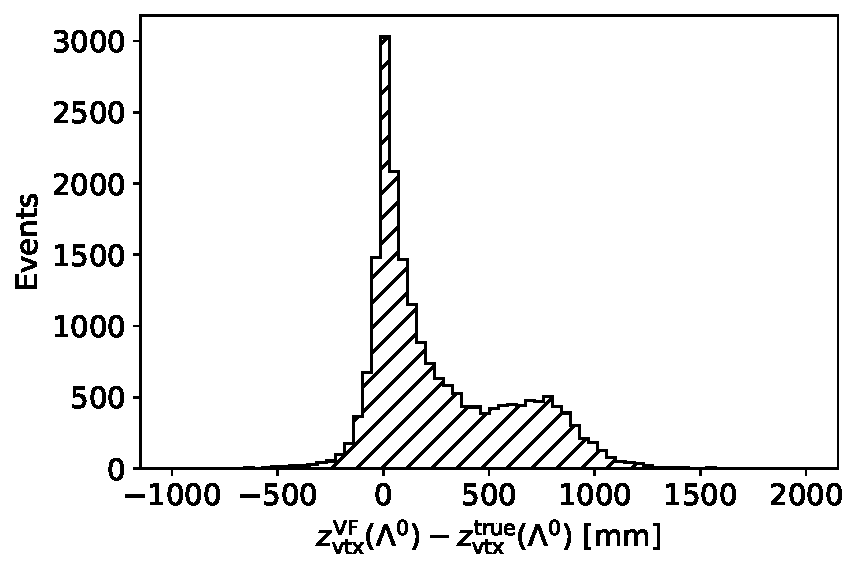
\includegraphics[width=\textwidth]{graphics/03-vertex_reconstruction/Lambda_endvertex_bias_z.pdf}
		\caption{}
		\label{fig:3:lz_endvertex_bias_linear}
	\end{subfigure}
	\begin{subfigure}{.45\textwidth}
		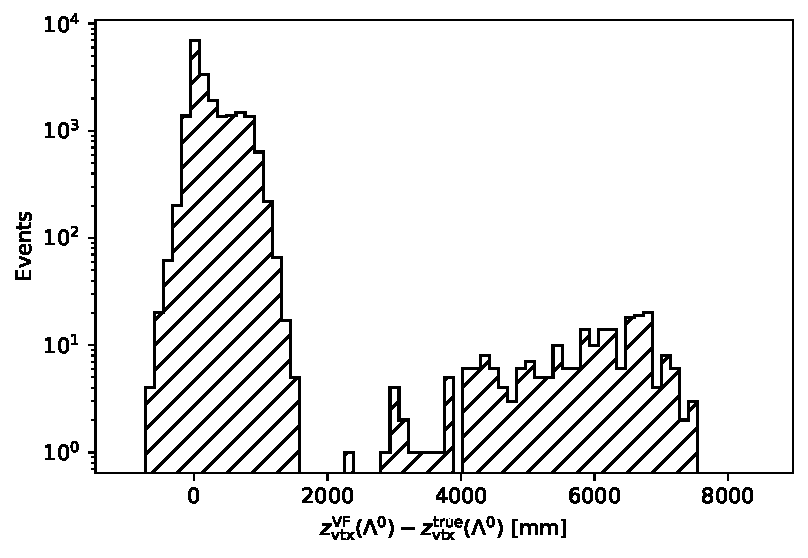
\includegraphics[width=\textwidth]{graphics/03-vertex_reconstruction/Lambda_endvertex_bias_z_log.pdf}
		\caption{}
		\label{fig:3:lz_endvertex_bias_log}
	\end{subfigure}
	\caption{Distribution of $z_\text{vtx}^\Lambda$ bias in linear \textit{(a)} and logarithmic \textit{(b)} scales for simulated \demonstratorshort events after all selection steps.}
	\label{fig:3:lz_endvertex_bias}
\end{figure}

The distribution of $z_\text{vtx}^\Lambda$ residuals for simulated signal events is shown in Figure \ref{fig:3:lz_endvertex_bias_linear}.
Its shape is distinctly non-gaussian, with a second core towards the positive end of the axis counterbalancing the expected $\approx 0$ peak, confirming the presence of a median bias of $\approx \SI{14}{\centi\meter}$. This number is of course much lower than the $\approx \SI{40}{\centi\meter}$ median bias of Vertex-Fitter-converging events quoted in Table \ref{tab:3:xyz_VF_performances}. Here not only am I directly selecting $z_\text{vtx}^\Lambda > \SI{5}{\meter}$, which reduces the extent of possible vertex bias given the position of the T stations around \SI{8}{\meter}, but many selection steps are also in place to skim out most badly reconstructed events.

\subsection{Ghost vertex events}
\label{sec:3:ghost_vertex}

The positive bias core can be interpreted as a mistake the vertexing algorithm commits when confronted with a specific decay geometry.
When the \lambdadecay decay plane closely aligns with the $xz$ bending plane, the bending induced by the magnet can produce either \textit{opening} or \textit{closing} tracks (depicted in the top and bottom diagrams respectively in Figure \ref{fig:3:horizontality_explanation}).
In the latter case the tracks will cross again at $z>z_\text{vtx}^\Lambda$;
if $y$ displacement is sufficiently small, the algorithms may converge on this <<ghost>> vertex instead of the real one.
This problem only affects physics analysis with T tracks as that's the only track classification for which the production vertex can be located after the dipole magnet, and thus the only case where the double crossing can occur.

%\begin{figure}[t]
%	\centering
%	\begin{subfigure}{.45\textwidth}
%		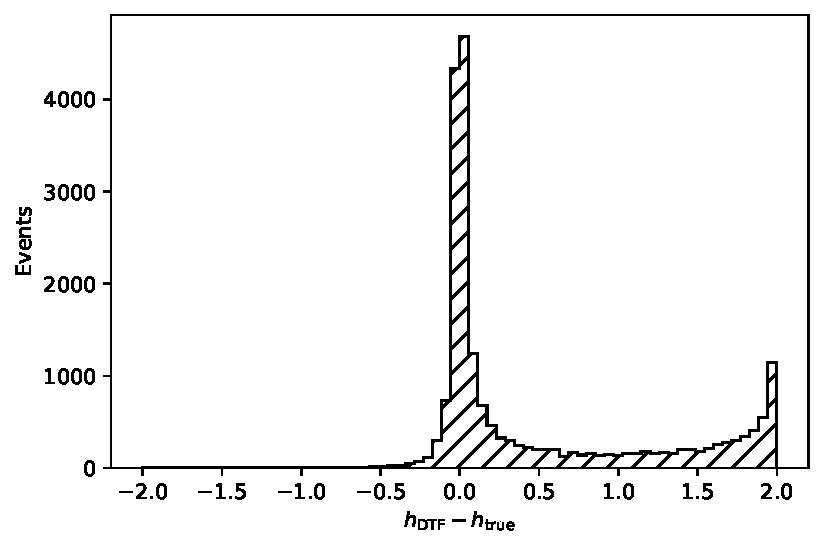
\includegraphics[width=\textwidth]{graphics/03-vertex_reconstruction/Lambda_horizontality_bias.pdf}
%		\caption{}
%		\label{fig:3:horizontality_bias}
%	\end{subfigure}
%	\begin{subfigure}{.45\textwidth}
%		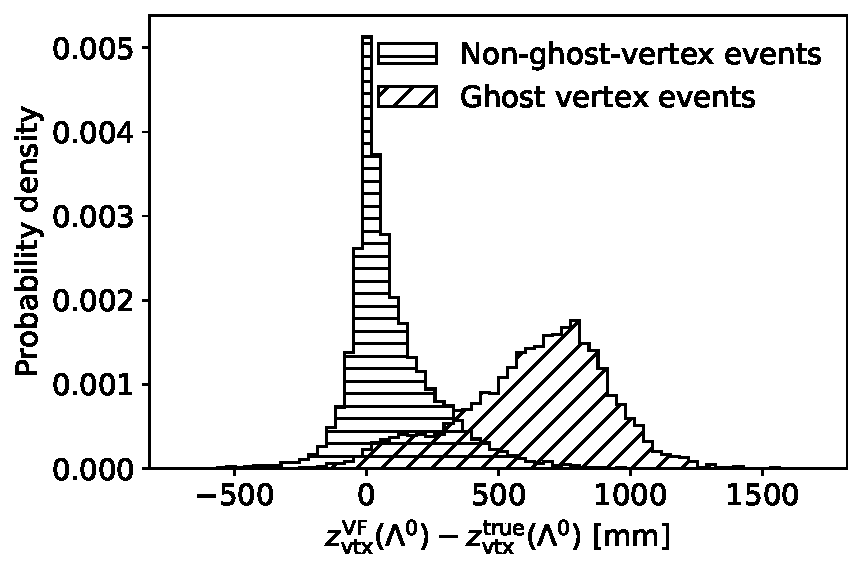
\includegraphics[width=\textwidth]{graphics/03-vertex_reconstruction/lambda_endvertex_z_bias_vs_horizontality_bias.pdf}
%		\caption{}
%		\label{fig:3:lz_endvertex_bias_vs_horizontality_bias}
%	\end{subfigure}
%	\caption{\textit{(a)} Bias in horizontality (as defined in \eqref{eq:3:horizontality}) of \lambdadecay decays from simulated \demonstratorshort events. Bias is obtained as the difference between $h_\text{DTF}$ (computed with Decay Tree Fitter momenta with \jpsi and \lz mass constraints) and $h_\text{true}$ (computed with true momenta). \textit{(b)} Distribution of $z_\text{vtx}^\Lambda$ bias for events with horizontality bias $<1$ (\textit{horizontal hatching}) and $\geq 1$ (\textit{diagonal hatching}).}
%\end{figure}

\begin{figure}[t]
	\centering
	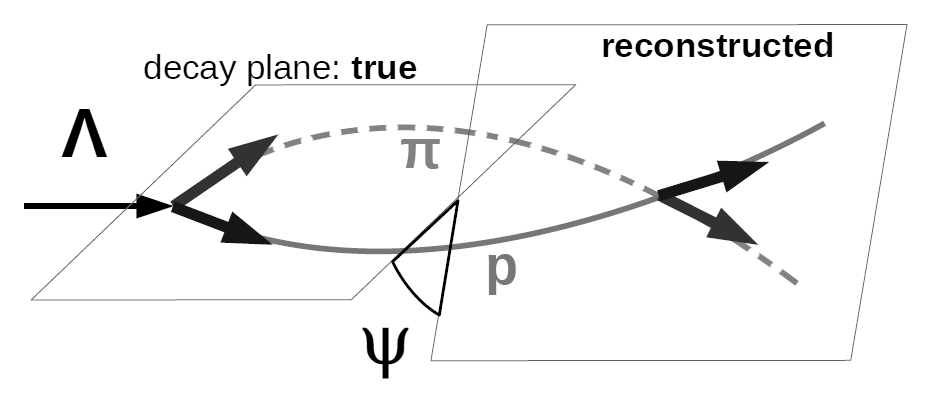
\includegraphics[width=.7\textwidth]{graphics/03-vertex_reconstruction/psi_diagram.png}
	\caption{Definition of angle $\psi$ as the angle between reconstructed and true \lambdadecay decay planes.}
	\label{fig:3:psi_explanation}
\end{figure}

To test out this hypothesis we define the auxiliary variable $\vec{a}$ as the cross product between proton and pion momenta at production vertex:
\begin{equation}
\vec{a} \coloneqq \vec{p}_p \times \vec{p}_\pi.
\end{equation}
This vector is perpendicular to the \lambdadecay decay plane, a property which allows us to compute angle $\psi$ between true and reconstructed decay planes, depicted in Figure \ref{fig:3:psi_explanation}, as the angle between $\vec{a}^\text{true}$ and $\vec{a}^\text{DTF}$ (the latter resulting from DTF momenta with \jpsi and \lz mass constraints):
\begin{equation}
\psi = \arccos{\left( \hat{a}_\text{true} \cdot \hat{a}_\text{reco} \right)}.
\label{eq:3:psi}
\end{equation}

\begin{figure}[t]
	\centering
	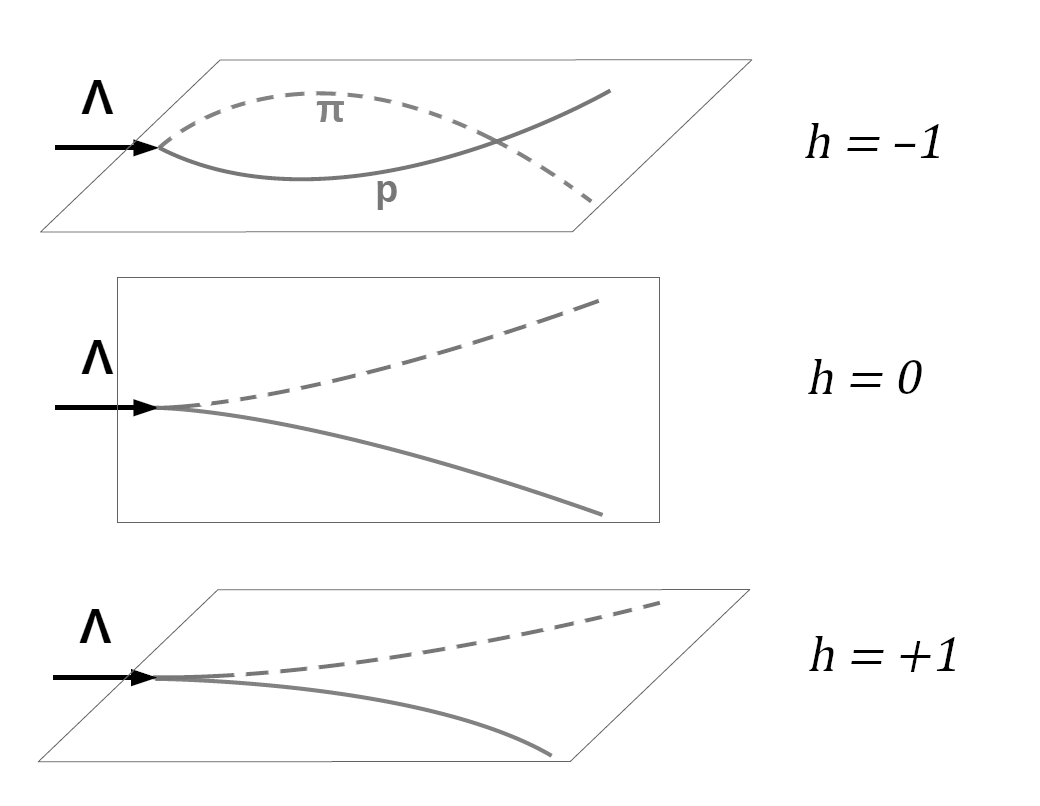
\includegraphics[width=.7\textwidth]{graphics/03-vertex_reconstruction/horizontality_illustration_bw.png}
	\caption{Depiction of three \lambdadecay configurations and the associated horizontality values. The horizontal planes in the top and bottom diagrams are aligned to the LHCb $xz$ plane, the vertical plane in the middle diagram to the $yz$ plane.}
	\label{fig:3:horizontality_explanation}
\end{figure}


We also define the \textit{horizontality} of a \lambdadecay event as follows:
\begin{equation}
h = \sign{\left(\Lambda^0_\text{PID}\right)} \sign{\left(B_y\right)}~\frac{a_y}{\lvert \vec{a} \rvert},
\label{eq:3:horizontality}
\end{equation}
where $\sign{\left(B_y\right)}$ is the dipole magnet polarity\footnote{The LHCb dipole magnet polarity is reversed roughly twice per month to allow for studies on decay asymmetries \cite{Vesterinen:1642153}. The $B_y > 0$ configuration is conventionally known as \textit{magnet up} polarity, $B_y < 0$ as \textit{magnet down}.}
and $\sign{\left(\Lambda^0_\text{PID}\right)}$ is the sign of the PDG Monte Carlo particle numbering scheme of the mother particle ($+1$ for $\Lambda^0$, $-1$ for $\bar{\Lambda}^0$) \cite{PDG}.
Decays with $h=\pm1$ lie exactly on the $xz$ bending plane, $h=-1$ events having closing $p\pi^-$/$\bar{p}\pi^+$ tracks and $h=+1$ events having opening tracks, while $h=0$ events lie on the $yz$ plane (the three cases are represented in Figure \ref{fig:3:horizontality_explanation}).

\begin{figure}[t]
	\centering
	\begin{subfigure}{.45\textwidth}
		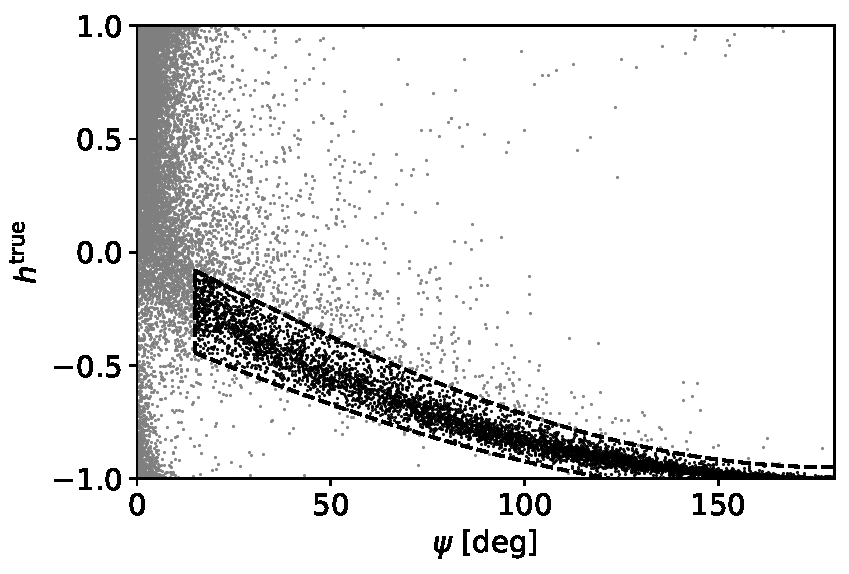
\includegraphics[width=\textwidth]{graphics/03-vertex_reconstruction/psi_vs_htrue.pdf}
		\caption{}
		\label{fig:3:psi_vs_htrue}
	\end{subfigure}
	\begin{subfigure}{.45\textwidth}
		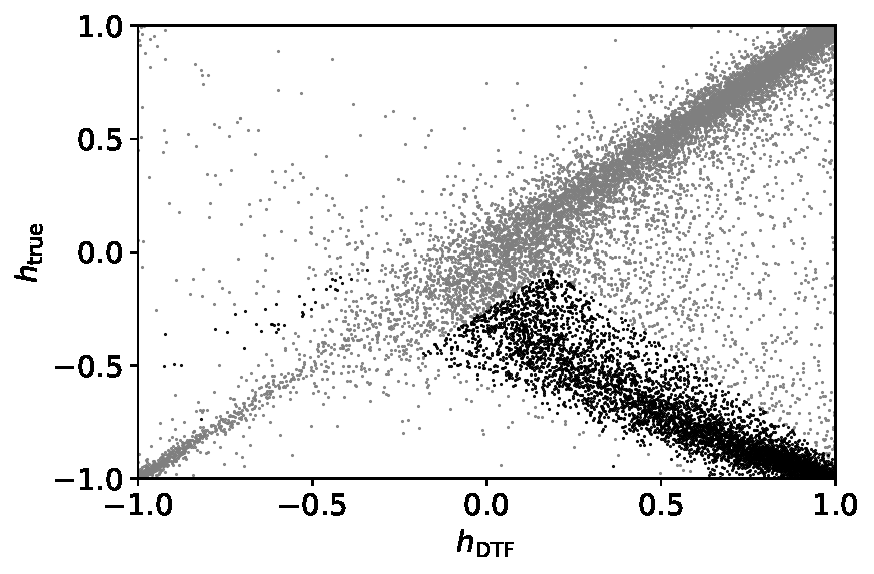
\includegraphics[width=\textwidth]{graphics/03-vertex_reconstruction/hreco_vs_htrue.pdf}
		\caption{}
		\label{fig:3:hreco_vs_htrue}
	\end{subfigure}
	\caption{\textit{(a)} Distribution of simulated \demonstratorshort events as function of angle $psi$ defined as \eqref{eq:3:psi} and true horizontality $h$ defined as \eqref{eq:3:horizontality}. The \textit{dashed lines} demarcates the ghost vertex locus of points defined in \eqref{eq:3:psih_banana}: events inside the region are marked in \textit{black}. All selection steps are applied. \textit{(b)} Distribution of the same events as function of true and reconstructed horizontality (the latter computed using momenta from the Decay Tree Fitter with \jpsi and \lz mass constraints).}
\end{figure}

The simplest case resulting in a ghost vertex is an opening-track \lambdadecay event fully lying on the $xz$ plane, whereby $y$ track distance is $\approx 0$ throughout the particle lines of flight and the second crossing of the tracks is chosen as the reconstructed vertex;
in such a case $h_\text{true} = -1$, $h_\text{DTF}=+1$ and $\psi = \pi$.
Due to poor momentum resolution at the VF level, which fixes the vertex positions for the following DTF refits, this issue affects many more $h_\text{true} < 0$ topologies.
This is clearly visible in Figure \ref{fig:3:psi_vs_htrue}: the $h_\text{true} < 0$, $\psi \leq 15$ deg region is depleted in favour of an arm-like structure stretching to high $\psi$ values.
No equivalent pattern for $h_\text{true} > 0$ is present because the vertex scan is performed starting from the T station measurements and moving upstream, converging on the first local minimum encountered;
thus it's very unlikely for opening-track events to be reconstructed as closing-track events by selecting an upstream ghost vertex.

To study the impact of ghost vertex events, I have isolated the above structure by parameterizing the locus of points
\begin{equation}
	\big\{ \left(\psi, h_\text{true} \right) \in \mathbb{R}^2
	: 
	\psi \geq 15\,\text{deg}
	\land
	f_\text{bottom}(\psi) \leq h_\text{true} \leq f_\text{top}(\psi)
	\big\},
	\label{eq:3:psih_banana}
\end{equation}
within the ad hoc horizontality region
\begin{subequations}
\begin{align}
	f_\text{top}(\psi) &= \frac{1}{20} - \sin\frac{\psi \left[\text{rad}\right]}{2}, \\
	f_\text{bottom}(\psi) &= - \frac{2}{25} - \sin\left(
	\frac{\pi}{12}
	-
	\frac{17}{40} \psi \left[\text{rad}\right]
	\right).
\end{align}
\end{subequations}
Events satisfying these requirements amount to $31.6\%$ of the total simulated sample after all selection steps applied.
Figure \ref{fig:3:hreco_vs_htrue} highlights the isolated events in the $h_\text{true}$--$h_\text{DTF}$ plane, showing that the vast majority of them are $h_\text{true} < 0$ events reconstructed as $h_\text{DTF} > 0$ events\footnote{A pocketful of events are located in the bottom left quadrant, though hard to see due to the meager number. These are rare cases where reconstructed horizontality is lower than the true value due to the low momentum resolution of T tracks.}.

\begin{figure}[t]
	\centering
	\begin{subfigure}{.45\textwidth}
		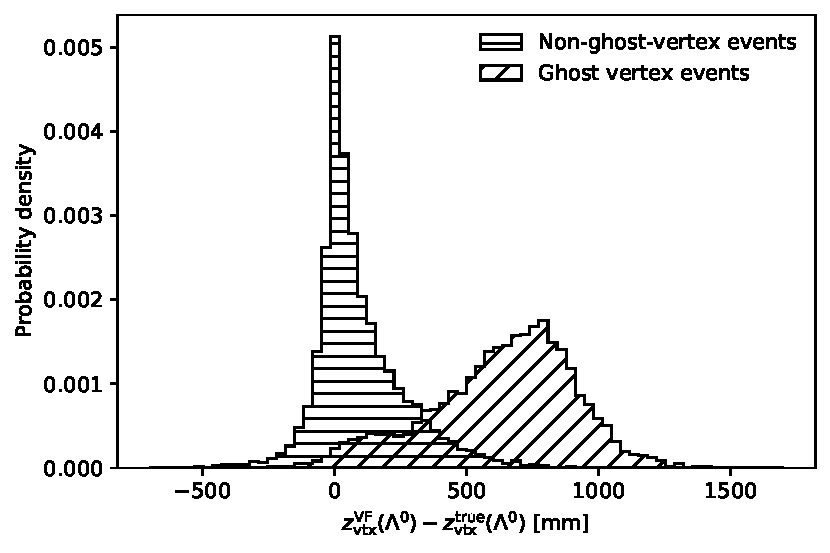
\includegraphics[width=\textwidth]{graphics/03-vertex_reconstruction/lambda_endvertex_z_bias_vs_ghost_vertex.pdf}
		\caption{}
		\label{fig:3:bias_without_ghost_vertex}
	\end{subfigure}
	\begin{subfigure}{.45\textwidth}
		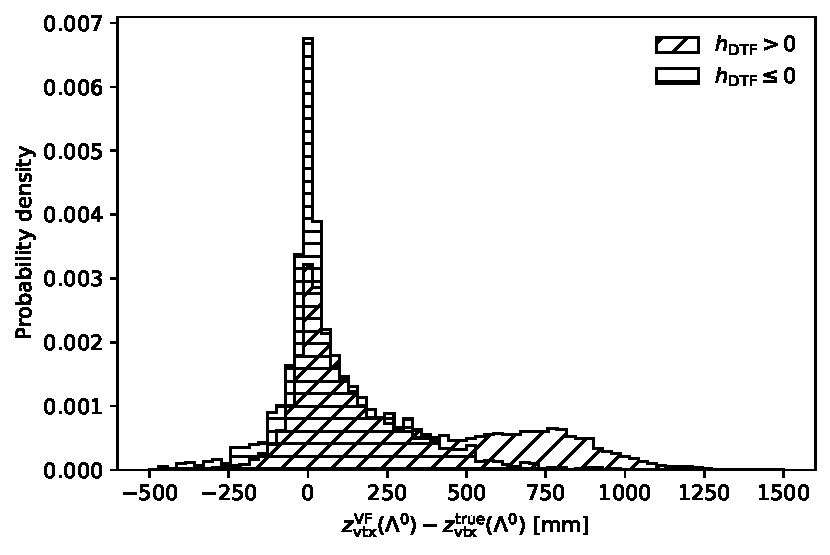
\includegraphics[width=\textwidth]{graphics/03-vertex_reconstruction/lambda_endvertex_z_bias_vs_reco_horizontality.pdf}
		\caption{}
		\label{fig:3:bias_without_positive_hDTF}
	\end{subfigure}
	\caption{Normalized distributions of $z_\text{vtx}^\Lambda$ bias for simulated \demonstratorshort events with all selection steps applied: \textit{(a)} without (\textit{horizontal hatching}) and with (\textit{diagonal hatching}) \lz ghost vertex, as selected in Figure \ref{fig:3:psi_vs_htrue}; \textit{(b)} with $h_\text{DTF} > 0$ (\textit{horizontal hatching}) and  $h_\text{DTF} \leq 0$ (\textit{diagonal hatching}), using DTF momenta with \jpsi and \lz mass constraints.}
%	\label{fig:3:bias_in_isolated_events}
\end{figure}

%A sufficiently small $y$ track distance is required for the Vertex Fitter to equivocate the ghost vertex for the real one, otherwise the event will not converge in the $yz$ plane.
%It follows that the signature for a ghost vertex event is a difference of $\approx 2$ between the reconstructed horizontality $h_\text{DTF}$ (using DTF momenta with \jpsi and \lz mass constraints) and true horizontality $h_\text{true}$, i.e. $h=-1 \rightarrow +1$.
%%A horizontality bias $\Delta h \coloneqq h_\text{reco} - h_\text{true} > 1$ thus becomes the signature of a ghost vertex \lambdadecay event.
%
%Figure \ref{fig:3:horizontality_bias} shows the $\Delta h \coloneqq  h_\text{DTF} - h_\text{true } > 1$ distribution for signal \lambdadecay events, highlighting a strong asymmetry between a large number of $\Delta h \approx 2$ events (closing to opening) and almost no $\Delta h \approx -2$ event (opening to closing).
%To isolate ghost vertex events I opted for a conservative $\Delta h > 1$ cut;
%this leaves out some events with double crossing in the $xz$ plane, such as those with $h_\text{true} = 0-\varepsilon_1 \rightarrow h_\text{DTF} = 0+\varepsilon_2$, but it's functional for a first look at the effect of ghost vertex reconstruction.

%As per Figure , this issue affects $\approx 25\%$ of reconstructed \demonstratorshort events, most of those being $\Delta h \approx 2$ events (from $h=-1$ to $h=+1$), with almost no event with $\Delta h < -1$.

The \lz decay vertex residual distributions shown in Figure \ref{fig:3:bias_without_ghost_vertex} confirm that ghost vertex events are largely responsible for the high-bias core observed in Figure \ref{fig:3:lz_endvertex_bias_linear}.
Some asymmetry effects are still visible in the distribution without ghost vertices, with a leftover median bias of $\approx \SI{5.2}{\centi\meter}$.
This suggests that further distorsion effects may be in place either in track reconstruction or in the fitting process and further investigation is warranted.

%%Isolating $\Delta h \geq 1$ events and studying their $z_\text{vtx}^\Lambda$ bias distributions (), it becomes clear that they 
%Significant asymmetry effects are , which is still skewed towards positive bias.
%While not ideal, this is somewhat expected given that the Vertex Fitter algorithm scans for candidate vertices starting from the first measurement position (i.e. the T1--T3 stations) and moving upstream.

Ongoing studies conducted by the Milan and Valencia LHCb research groups suggest that ghost vertex convergence in double-crossing tracks can be tempered by tweaking the initial vertex seed.
The choice of seed defines the starting point for the Vertex Fitter algorithm:
early results show that overriding the seeding process (see Section \ref{sec:3:seeding}) to use the true \lambdadecay vertex as seed helps direct the VF towards the absolute $\chi^2$ minimum and reduces the ghost vertex core seen in Figure \ref{fig:3:bias_without_ghost_vertex}.
A similar result could be achieved without access to Monte Carlo information by performing several vertex fits with seeds across the $z$ range and implementing selection criteria to choose the best vertex among the ones found.

An alternative, more drastic approach would be to only retain \lambdadecay events with $h_\text{DTF} \leq 0$. As seen from Figure \ref{fig:3:hreco_vs_htrue}, this rejects virtually all ghost vertex events and yields an even lower median bias of $\approx \SI{2.5}{\centi\meter}$ with a single cut on reconstructed variables (see Figure \ref{fig:3:bias_without_positive_hDTF}).
The ensuing 89\% loss in \demonstratorshort signal makes this solution impractical with Run 2 data, but viable as a last resort on the projected \SI{50}{\per\femto\barn} dataset at the end of Run 4.

For the purposes of this thesis, no cut on ghost vertex events is applied.
Their impact on the resolutions for the proton angular distribution in \lambdadecay decays is studied in Section \ref{sec:5:resolution_after_ghost}.

\subsection{Very high bias events}

\begin{figure}[t]
	\centering
	\begin{subfigure}{.45\textwidth}
		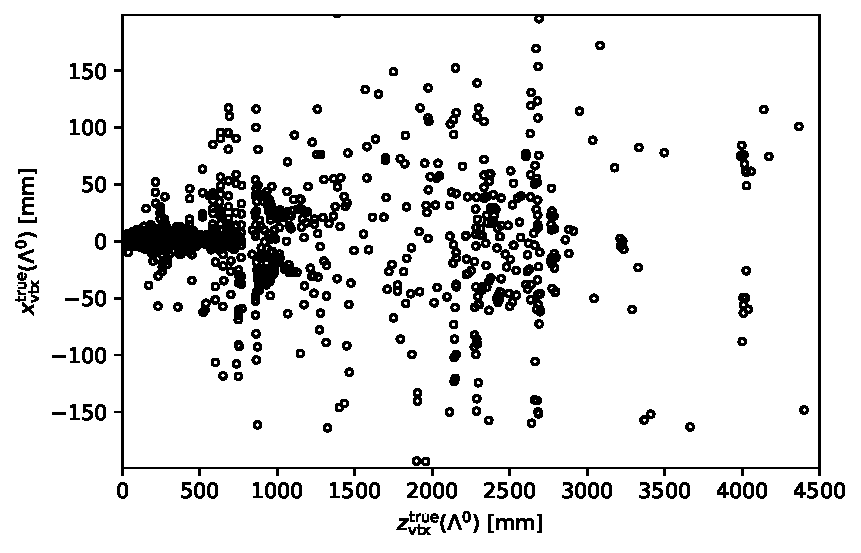
\includegraphics[width=\textwidth]{graphics/03-vertex_reconstruction/bump_Lambda_true_endvertex_z_vs_x.pdf}
		\caption{}
		\label{fig:3:bump_true}
	\end{subfigure}
	\begin{subfigure}{.45\textwidth}
		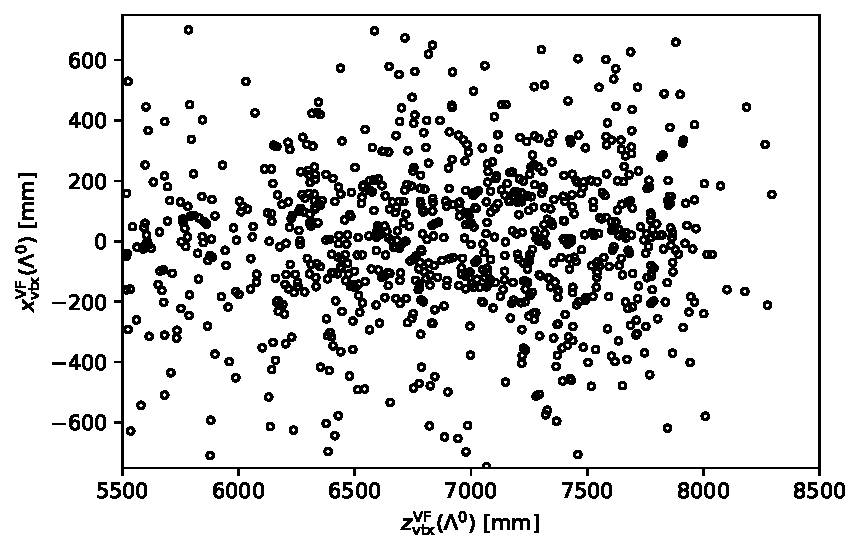
\includegraphics[width=\textwidth]{graphics/03-vertex_reconstruction/bump_scatter_Lambda_endvertex_z_vs_x.pdf}
		\caption{}
		\label{fig:3:bump_reco}
	\end{subfigure}
	\caption{Distribution of simulated \demonstratorshort events (only prefilters applied) with $z_\Lambda^\text{VF} - z_\Lambda^\text{true} \geq \SI{2.0}{\meter}$ as function of true \textit{(a)} and reconstructed \textit{(b)} $x^\Lambda_\text{vtx}$ and $z_\text{vtx}^\Lambda$. This corresponds to a top view of true and reconstructed \lz decay vertices.}
	\label{fig:3:bump}
\end{figure}

Most \demonstratorshort events, even those with ghost vertex reconstruction, still maintain a limited $\lesssim \SI{1.0}{\meter}$ bias on $z_\text{vtx}^\Lambda$.
A smaller substructure with $\geq \SI{2.0}{\meter}$ bias (median bias $\approx \SI{6.0}{\meter}$) emerges when plotting the distribution in logarithmic scale, as seen in Figure \ref{fig:3:lz_endvertex_bias_log}.
These events only amount to $\approx 0.5\%$ of the sample after the full selection process.
The fraction rises to $\approx 1.7\%$ when only the loose prefiltering selection from Section \ref{sec:prefilter} is applied, meaning that most of these events are already rejected in the following selection steps.
To maximize statistics, I studied this <<very high bias>> class of events omitting said steps.

Figure \ref{fig:3:bump_true} provides a top view of the $\Lambda^0$ decay vertices for these events, showing the distribution of true $z_\text{vtx}^\Lambda$ and $x_\text{vtx}^\Lambda$.
Most $\Lambda^0$ in high bias events decay in the earlier sections of the detector ($z<\SI{3.0}{\meter}$);
the high spatial concentration in specific regions of the $xz$ plane, such as the <<wings>> around $z\approx \SI{1.0}{\meter}$, as well as the consistency between the placement of these structures and the location of the different LHCb subdetectors (cf. Figure \ref{fig:2:lhcb_diagram}), suggest that they may be the result of interaction with the material.

No dedicated veto on reconstructed variables is possible to filter this class of events:
Figure \ref{fig:3:bump_reco} shows that the $\Lambda^0$ vertices are reconstructed in seemingly arbitrary positions.
Their impact on the overall performance on signal is nevertheless neglectable.

\section{Summary and closing remarks}
\label{sec:3:cap3_conclusions}

Vertex reconstruction involving T tracks has never been the subject of in-depth scrutiny due to the rare usage of said class of tracks in physics analyses.
Given the number of different topics tackled in the present chapter, in this section I offer a more succint recount of the main findings and outline the solutions I have adopted for the remainder of this thesis.

One major challenge to a competitive measurement of \lz electromagnetic dipole moments using the exclusive \demonstratorfull decay is the $\lesssim 50\%$ efficiency of the \lz and \lbz vertex reconstruction process, effectively halving the potential signal yield.
Topological studies on reconstruction of the \lambdadecay decay in non-converged events expose that the failure of the Vertex Fitter algorithm is caused by the oscillation of the \lz candidate vertex throughout the iterating process, preventing fulfilment of either of convergence conditions \eqref{eq:cond_conv_1} and \eqref{eq:cond_conv_2}.

Another widespread characteristic of non-converged events is the discrepancy in $z$ coordinate between the point of closest track distance in the $xz$ plane (where tracks are curved due to the magnetic field) and the crossing track point in the $yz$ plane (where tracks are approximately straight lines).
The distance between the two, sometimes exceeding \SI{1}{\meter}, is consistent with the scale of candidate vertex oscillation in the VF iterating process.
This suggests that, at least for a portion of non-converged events, the Vertex Fitter locates two irreconcilable vertex candidates in the $xz$ and $yz$ track propagation planes and is unequipped to choose one over the other.

To address this problem, I developed and implemented a threefold refit process that sequentially favours $yz$, $xz$ and $xy$ propagation planes by increasing the complementary uncertainty ($\sigma_x$, $\sigma_y$ and $\sigma_z$ respectively) in the vertex covariance matrix.
This results in a a $+26.4\%$ increase in signal statistics compared to only using the standard Vertex Fitter, recovery roughly one quarter of all non-converged \demonstratorshort events.

The reason for the $xz$-$yz$ discrepancy, and thus of the oscillation at the heart of vertexing failure, is currently unknown.
However, an observed systematic underestimation of $p_z$ for pion tracks in non-converged events suggests it could be linked to poor momentum measurement at T station level.
The negative $p_z$ bias affects recovered events as well, imprinting a median bias on $z_\text{vtx}^\Lambda$ roughly \SI{20}{\centi\meter} greater than standard converged events.
Recovered events also have generally worse $\tilde{\chi}^2_\text{vtx}$; dedicated studies on algorithm performances point to this being a problem with the event themselves being difficult to fit, rather than to issues with the algorithms.

Given the importance of \lambdadecay vertex bias for the measurement of the \lz dipole moments, I also investigated the reconstruction of the aforementioned decay and identified two main classes of biased events.
<<Ghost vertex>> events are a byproduct of the action of the dipole magnet, which bends proton and pion tracks into a second crossing point mistakenly chosen as the $p\pi^-$ production vertex.
These events comprise almost one third of the full dataset and contribute a median \SI{70}{\centi\meter} bias in $z_\text{vtx}^\Lambda$;
their effect on proton angular resolution is the focus of a study in Section \ref{sec:5:resolution_after_ghost}.
<<Very high bias>> events contribute a much larger median bias of \SI{6}{\meter}, but their impact on the \demonstratorshort analysis is considered to be neglectable, as they only amount to 0.5\% of the simulated sample after the full selection process.